\documentclass{llncs}

% \usepackage{showframe}

\usepackage{amssymb}
\usepackage[fleqn]{amsmath}
\usepackage{url}
\usepackage{graphicx}
\usepackage{float}
\usepackage{listings}
\usepackage[ruled,vlined]{algorithm2e}
\usepackage{mathtools}
\usepackage[rightcaption]{sidecap}
\usepackage{multicol}
\usepackage{colortbl}
\usepackage{booktabs}
\usepackage{framed}
\usepackage{tikz}
\usepackage{pdflscape}
\usepackage{afterpage}

\usetikzlibrary{shapes, shapes.multipart, arrows, positioning, calc}

\newcommand{\match}{\mathit{match}}
\newcommand{\timeSlot}{\mathit{timeSlot}}
\newcommand{\state}{\mathit{state}}
\newcommand{\change}{\mathit{change}}
\newcommand{\totalChanges}{\mathit{totalChanges}}
\newcommand{\totalBoatChanges}{\mathit{totalBoatChanges}}
\newcommand{\modMatch}{\mathit{modMatch}}
\newcommand{\position}{\mathit{position}}
\newcommand{\imbalance}{\mathit{imbalance}}
\newcommand{\maxImbalance}{\mathit{maxImbalance}}
\newcommand{\timeVar}{\mathit{time}}

\newcommand{\START}{\textnormal{\textsc{Start}}}
\newcommand{\FIRST}{\textnormal{\textsc{First}}}
\newcommand{\MID}{\textnormal{\textsc{Mid}}}
\newcommand{\LAST}{\textnormal{\textsc{Last}}}
\newcommand{\END}{\textnormal{\textsc{End}}}
\newcommand{\BYE}{\textnormal{\textsc{Bye}}}

\newcommand{\eachOccursExactlyOnce}{\mathrm{eachOccursExactlyOnce}}
\newcommand{\allDifferent}{\mathrm{allDifferent}}
\newcommand{\validStateSequence}{\mathrm{validStateSequence}}
\newcommand{\minimise}{\mathrm{minimise}}
\newcommand{\maximum}{\mathrm{maximum}}

\DeclarePairedDelimiter\abs{\lvert}{\rvert}

\newcommand\nldots{\,\hbox to 0.8em{.\hss.\hss.}\,}

\sidecaptionvpos{table}{c}

\definecolor{uofgheather}{rgb}{0.356863, 0.32549, 0.490196}
\definecolor{uofgaquamarine}{rgb}{0.603922, 0.72549, 0.678431}
\definecolor{uofgslate}{rgb}{0.309804, 0.34902, 0.380392}
\definecolor{uofgrose}{rgb}{0.823529, 0.470588, 0.709804}
\definecolor{uofgmocha}{rgb}{0.709804, 0.564706, 0.47451}

\definecolor{uofglawn}{rgb}{0.517647, 0.741176, 0}
\definecolor{uofgcobalt}{rgb}{0, 0.615686, 0.92549}
\definecolor{uofgturquoise}{rgb}{0, 0.709804, 0.819608}
\definecolor{uofgsunshine}{rgb}{1.0, 0.862745, 0.211765}
\definecolor{uofgpumpkin}{rgb}{1.0, 0.72549, 0.282353}
\definecolor{uofgthistle}{rgb}{0.584314, 0.070588, 0.447059}
\definecolor{uofgpillarbox}{rgb}{0.701961, 0.047059, 0}
\definecolor{uofglavendar}{rgb}{0.356863, 0.301961, 0.580392}

\begin{document}

\title{Constructing Sailing Match Race Schedules: Round-Robin Pairing Lists}
\titlerunning{Match Race Scheduling}
%\toctitle{}
\author{Craig Macdonald \and Ciaran McCreesh \and Alice Miller \and Patrick Prosser}
\institute{University of Glasgow, Glasgow, Scotland \\ \email{patrick.prosser@glasgow.ac.uk}}
\authorrunning{Macdonald, McCreesh, Miller, Prosser}
\maketitle

\begin{abstract}
We present a constraint programming solution to the problem of generating round-robin schedules for sailing match races. Our schedules satisfy the critria published by the International Sailing Federation (ISAF) governing body for match race pairing lists. We show that some published ISAF schedules are in fact illegal, and present
corresponding legal instances and schedules that have not previously been published. Our schedules
can be downloaded as blanks, then populated with actual competitors and used in match racing competitions.
\end{abstract}

\section{Introduction}

This work describes a round-robin competition format that arises from sailing, known as match
racing. Competitors, i.e.\ \emph{skippers}, compete against each other in a series of matches taking
place in rounds, known as \emph{flights}.  A match is composed of two skippers, with each skipper in
a boat on their own. Skippers in a match set off together, one on the port side, the other starboard,
and first home wins that match. Criteria published by the International Sailing Federation (ISAF)
dictate what makes a legal match race schedule and what should be optimised. This is a rich set of
criteria, 13 in all, and as far as we know, all published schedules have been produced by hand. This
is a daunting task. A close inspection of these schedules reveals that most are illegal, violating
many of the match race scheduling criteria, many schedules are missing, and some that are legal are
far from the ISAF definition of optimality.

This paper describes the scheduling problem. We present a constraint programming solution and
document how this model was constructed incrementally. We believe this illustrates how adaptable
constraint programming is: a robust model can be developed incrementally to address all of the
required criteria. Our schedules are then constructed in a sequence of stages, not dissimilar to the
hybrid and decomposition based approaches by Lombardi and Milano \cite{lombardi2012}. Some ISAF
published schedules are presented along with some of our own, some of these being new.  These
schedules are essentially blank forms, made available to event organisers, which can be filled in
with names of actual competitors, i.e.\ these schedules are reusable.

The paper is organised as follows: we introduce the 13 match racing criteria, then explain the
constraint models and four stages of schedule construction, and then schedules are presented. We
finish with discussion and a conclusion.

\section{Problem Definition: Round-Robin Pairing Lists}\label{sec:definition}

The guidelines for running match racing events~\cite{isaf} places a number of criteria on how the
competing skippers are scheduled into flights and matches, known as pairing lists. Several of these
criteria are applicable when the number of skippers exceeds the number of available boats, in which
case skippers have to change in and out of boats, and are allowed time in the schedule to check and
fine-tune the boat they change into. Typically, matches set off at 5 minute intervals with each
match taking about 20 minutes. Therefore, if we have 10 skippers and 10 boats we have 45 matches.
This results in 9 flights each of 5 matches.  Each flight takes about 50 minutes, so eight or nine
flights a day is a reasonable achievement for most events~\cite{isaf}. Consequently, the number of
boats and skippers involved is typically small.

The criteria for  match racing schedules (pairing lists) are given in ISAF ``International Umpires'
and Match Racing Manual'' \cite{isaf}, section M.2 ``Recommended Criteria for Round Robin Pairing
Lists'', and are detailed below.

\begin{framed}
\noindent Principal Criteria in Order of Priority:
\begin{enumerate}
\item[1.] Each skipper sails against each other skipper once.
\item[2*.] When skippers have an even number of matches, they have the same number of port and starboard
    assignments.
\item[3*.] When skippers have an odd number of matches, the first half of the skippers will have one
    more starboard assignment.
\item[4.] No skipper in the last match of a flight should be in the first match of the next flight.
\item[5.] No skipper should have more than two consecutive port or starboard assignments.
\item[6.] Each skipper should be assigned to match 1, match 2, etc. in a flight as equally as possible.
\item[7.] In flights with five or more matches, no skipper should be in the next-to-last match in a
    flight and then in the first match of the next flight.
\item[8.] If possible, a skipper should be starboard when meeting the nearest lowest ranked skipper
    (i.e.\ \#1 will be starboard against \#2, \#3 will be starboard against \#4).
\item[9.] Close-ranked skippers meet in the last flight.
\item[10.] Minimise the number of boat changes.
\item[11.] Skippers in the last match of a flight do not change boats.
\item[12.] Skippers in new boats do not sail in the first match of the next flight.
\item[13.] Skippers have a reasonable sequence of matches and blanks.
\end{enumerate}
Note that criteria~10, 11 and~12 only apply when there are fewer boats than skippers; 11 and~12
override~6 when changes are required, and~13 applies when there are more boats than skippers.
\end{framed}

We have rephrased criteria~2 and~3 (denoted *) to clarify an error in the manual \cite{isaf}. Note
that the order of matches within a flight is significant and is constrained, as is the order of
flights within a schedule and the position of skippers within a match. This permits fair schedules
that provide the sufficient changeover time for skippers changing boats, etc.

Criteron~6 allows us to measure the \emph{balance} of a schedule. Perfect balance would be when a skipper has as many matches in first position in flights as in second position in flights, and so on. For example, if we had 9 skippers and 8 boats, each skipper would have 8 matches and could be in the first, second, third or fourth match of a flight. In perfect balance, each of the 8 skippers would appear twice in each position. Balance is one of our optimisation criteria.

Criterion~13 uses the term \emph{blanks} where conventionally we use the term \emph{bye}. That is, a blank is a bye and a bye is a flight where a skipper does not compete (and is ashore).

Criterion~12 discusses boat changes: if in flight $i$ this skipper is not in a match (i.e. it is a
bye for this skipper) but is in a match in flight $i+1$ then he has to get into a boat, rearrange
all his kit and set the boat to his preference before racing commences, and this is a boat change. 

Next, we note that skippers can be ranked prior to an event, based on their performance in
previous events\footnote{\url{http://www.sailing.org/rankings/match/}}, which is used to seed the
skippers. The ordering of skippers within a match signifies their starting position (port or
starboard), as skippers allocated the starboard starting position gain a small competitive
advantage in that match---criterion~8 accomplishes the seedings.

Criterion~10 is ambiguous: this could be interpreted on a schedule basis: i.e.\ to minimise the
overall number of changes in the entire pairing list schedule; or alternatively as well as a fair,
but minimal number of changes across all skippers. In our work, we take the latter viewpoint.

There are some conflicts inherent in the criteria. Take criteria~4 and~11, assume we have 4 boats, and
in flight $i$ the last match is the pair of skippers ($x,y$). Criterion~11 dictates that skippers $x$
and $y$ must appear in the next flight, $i+1$, and criterion~4 that neither can be first in the next
flight. This forces skippers $x$ and $y$ to compete in flight $i+1$ as the last match, violating
criterion~1. Therefore, although not explicitly stated, it is not possible to satisfy every criteria
with fewer than 6 boats.

\section{The Constraint Models}\label{sec:models}

Our approach produces schedules in four stages. The first stage produces a schedule that respects
criteria~1, 4, 11 and~12, and minimises criteria~10 (boat changes). The second stage constructs a
schedule that respects criteria~1, 4, 11, 12 (again), has criterion~10 as a hard constraint generated
from first stage, and minimises criterion~6 (balance). This results in a schedule that attempts to
minimise boat changes \emph{and} balance. The third stage satisfies criterion~9, and is a simple
translation of the schedule produced in stage 2.  The final stage orients skippers within matches to
address criteria~2, 3, 5 and~8.

We now describe the constraint models and processes used in each stage. In the text below we assume
there are $n$ skippers and $b$ boats, with $m = b/2$ matches in a flight. In total there are $t =
n(n-1)/2$ matches and $f = \lceil n(n-1)/m  \rceil$ flights. We use the schedule in
Table~\ref{tab1}, for 7 skippers and 6 boats, to help illustrate the constraint models. 

\begin{SCtable}[1.8][tb]
    \setlength{\tabcolsep}{3pt}
    \begin{tabular}{cccc}
        \toprule
        Flight & \multicolumn{3}{c}{Matches} \\ \midrule
        0 & (0,1) & (2,3) & (4,5) \\
        1 & (0,2) & (4,6) & (1,5) \\
        2 & (2,6) & (0,5) & (1,3) \\
        3 & (5,6) & (0,3) & (1,4) \\
        4 & (3,5) & (1,6) & (2,4) \\
        5 & (3,6) & (0,4) & (2,5) \\
        6 & (3,4) & (1,2) & (0,6) \\ \bottomrule
    \end{tabular}
    \caption{A round-robin schedule with 7 skippers, 6 boats and 7 flights.  Skippers are numbered 0
        to 6. Note that the order of skippers within a flight is significant, as is position within
        a match (port or starboard). This schedule is the result of stages 1 and 2, and has yet to
        be renumbered and oriented (stages 3 and 4).} \label{tab1}
\end{SCtable}

\subsection{Stage 1: Minimising Boat Changes}

\paragraph{Modeling skippers:} The first thing we model, in the first half of
Figure~\ref{model:stage1}, is a skipper. Each skipper $\sigma$ has both a temporal view of their
schedule (``who, if anyone, am I racing in the match at time $t$?''), and a state view (``where am
I racing within flight $f$?'').  The temporal view is via the array $\timeSlot$ defined in
\eqref{var:timeSlot}. If variable $\timeSlot[{i}] = k$ and $k \geq 0$ then this skipper is in a
match with skipper~$k$ at time~$i$.

Variable $\state[{i}]$ \eqref{var:state} gives the state of this skipper in flight~$i$,
corresponding to time slots $\timeSlot[{m \cdot i}]$ to $\timeSlot[{m(i+1)-1}]$.
The cases in \eqref{C1} state that a skipper can be in a match in the first time slot in the flight,
or in the middle of the flight\footnote{i.e.\ not first and not last.}, or in the last time slot of
the flight. Alternatively, if all time slots in a flight are equal to $-1$ then the skipper is in a
bye (i.e. not in a match in this flight), and if all time slots in a flight are equal to $-2$ then
the skipper has finished all matches.

\begin{figure}[p]
\setlength{\mathindent}{1em}
\setlength{\abovedisplayskip}{0pt}
\setlength{\belowdisplayskip}{0pt}
\setlength{\abovecaptionskip}{0pt}
\begin{framed}
\begin{align}
    \intertext{A copy of these variables and constraints is created for each skipper $\sigma$:\smallskip}
    &\forall \tau \in \{0 \nldots t{-}1\}: \timeSlot[{\tau}] \in \{{-}2 \nldots t{-}1\} \setminus \{\sigma\} \label{var:timeSlot} \tag{V1} \\
    &\forall i \in \{0 \nldots f{-}1\}: \state[{i}] \in \{\FIRST,\MID,\LAST,\BYE,\END\} \label{var:state} \tag{V2} \\
    &\forall i \in \{0 \nldots f\}: \label{C1} \tag{C1} \\
    &\begin{alignedat}{3}
    &\hspace*{1em} \state[{i}] = \FIRST &\ &\Leftrightarrow&&\ \timeSlot[{m \cdot i}] \geq 0 \\
    &\hspace*{1em} \state[{i}] = \MID   &\ &\Leftrightarrow&&\ \exists j \in \{m \cdot i + 1 \nldots m \cdot (i + 1) - 2\} : \timeSlot[{j}] \geq 0 \\
    &\hspace*{1em} \state[{i}] = \LAST  &\ &\Leftrightarrow&&\ \timeSlot[m \cdot (i + 1) - 1] \geq 0 \\
    &\hspace*{1em} \state[{i}] = \BYE   &\ &\Leftrightarrow&&\ \forall j \in \{m \cdot i \nldots m \cdot (i + 1) - 1\} : \timeSlot[j] = -1 \\
    &\hspace*{1em} \state[{i}] = \END   &\ &\Leftrightarrow&&\ \forall j \in \{m \cdot i \nldots m \cdot (i + 1) - 1\} : \timeSlot[j] = -2
    \end{alignedat} \nonumber \\
    &\eachOccursExactlyOnce(\timeSlot, \{0, \nldots, n{-}1\} \setminus \{\sigma\}) \label{C2} \tag{C2} \\
    &\validStateSequence(\state) \label{C3} \tag{C3} \\[0.1cm]
    & \forall i \in \{0 \nldots f{-}2\}: \change[{i}] \in \{0,1\} \label{V3} \tag{V3} \\
    & \totalChanges \in \mathbb{N} \label{V4} \tag{V4} \\
    & \forall i \in \{0 \nldots f{-}2\}: \change[{i}] = 1 \Leftrightarrow \state[{i}] = \BYE \wedge \state[{i + 1}] \neq \BYE \label {C4} \tag{C4} \\
    & \totalChanges = \textstyle\sum \change \label{C5} \tag{C5}
\end{align}
\end{framed}\begin{framed}
\begin{align}
    \intertext{Match and temporal perspectives:\smallskip}
    & \forall i \in \{0 \nldots n{-}2\} : \forall j \in \{ i{+}1 \nldots n{-}1 \} : \nonumber \\
    & \hspace*{1em} \match[{i,j}] \in \{0 \nldots t{-}1\} \tag{V5} \label{V5} \\
    & \hspace*{1em} \match[{j,i}] \equiv \match[{i,j}] \nonumber \\
    & \hspace*{1em} \forall k \in \{0 \nldots t{-}1 \} : \nonumber \\
    & \hspace*{2em} \match[{i,j}] = k \Leftrightarrow \sigma[{i}].\timeSlot[{k}] = j \wedge \sigma[{j}].\timeSlot[{k}] = i \tag{C6} \label{C6} \\[0.1cm]
    & \forall i \in \{0 \nldots n{-}2\} : \forall j \in \{ i{+}1 \nldots n{-}1 \} \nonumber : \\
    & \hspace*{1em} \modMatch[{i,j}] \in \{0 \nldots f{-}1\} \label{V6} \tag{V6} \\
    & \hspace*{1em} \modMatch[{j,i}] \equiv \modMatch[{i,j}] \nonumber  \\
    & \hspace*{1em} \modMatch[{i,j}] = \match[{i,j}] / m \tag{C7} \label{C7} \\
    & \forall i \in \{0 \nldots n{-}1 \} : \allDifferent(\modMatch[{i}]) \tag{C8} \label{C8} \\[0.1cm]
    & \forall \tau \in \{0 \nldots t{-}1 \} : \nonumber \\
    & \hspace*{1em} \timeVar[{\tau}] \in \{(0,1) \nldots (n{-}2,n{-}1)\} \tag{V7} \label{V7} \\
    & \hspace*{1em} \forall i \in \{0 \nldots n{-}2\} : \forall  j \in \{ i{+}1 \nldots n{-}1 \} : \timeVar[{\tau}] = (i,j) \Leftrightarrow \match[{i,j}] = \tau \tag{C9} \label{C9} \\[0.1cm]
    & \totalBoatChanges = \textstyle\sum \sigma.\totalChanges \label{V8} \tag{V8} \\
    & \minimise(\totalBoatChanges) \label{C10} \tag{C10}
\end{align}
\end{framed}
\caption{Our constraint model, from a skipper perspective (top) and a match and temporal perspective
(below). The number of skippers is $n$, and $m$ is the number of matches in a flight. The number of
flights is $f = \lceil n(n-1)/m \rceil$, and there are $t = n(n-1)/2$ matches in
total.}\label{model:stage1}
\end{figure}

We must then ensure that each skipper $\sigma$ is in a match with all other skippers $\{0, \nldots,
n-1\} \setminus \{\sigma\}$. This is \eqref{C2}, which is enforced by imposing a global
cardinality constraint \cite{globCard} on the array $\timeSlot$.

\paragraph{State transitions:} The $\state$ variables are then used to impose match race criterion~4
(if last in flight $i$ then not first in flight $i+1$), criterion~11 (if last in flight $i$ then not
in a bye in flight $i+1$) and criterion~12 (if flight $i$ is a bye then flight $i+1$ is not first).
These criteria are imposed by \eqref{C3}, which is a deterministic finite automaton (DFA) constraint
\cite{Pesant04}. The transitions for the DFA are shown pictorially in Figure~\ref{skipper5}: arcs
represent a possible transition from one state to another. The DFA is encoded as a set of transition objects
$\langle q_{i},\iota,q_{j} \rangle$, where a transition is made from state $q_{i}$ to state $q_{j}$
when encountering input~$\iota$. In addition we specify the accepting states, which are all states
except the start state (white) and the bye state (pink).  This constraint also ensures that if a
skipper has finished all matches in flight $i$ (i.e.\ is in state $\END$) then that skipper will also have
finished all matches in flight $i+1$ (and so on).

Figure~\ref{skipper5} also shows the skipper-oriented variables and constraints corresponding to
skipper 5 in the schedule shown in Table~\ref{tab1}. The $\state$ array is presented as coloured boxes, and
below that is the $\timeSlot$ array. The arrows represent the channeling constraints \eqref{C1}. The
$\state$ array is coloured with green representing $\LAST$, yellow for $\MID$, blue for $\FIRST$,
red for $\LAST$ and (not shown) pink for $\BYE$. The schedule of Table~\ref{tab1} is reproduced with
the matches for skipper 5 emboldened.

\paragraph{Boat changes:} A boat change occurs when a skipper has been in a $\BYE$ state in flight
$i$ and then is in a match in the next flight $i+1$.  This is encoded using the array of zero/one
variables \eqref{V3}, and the constraint \eqref{C4}, and accumulated into $\totalChanges$
(\ref{V4},~\ref{C5}).

\begin{figure}[tb]
    \centering
    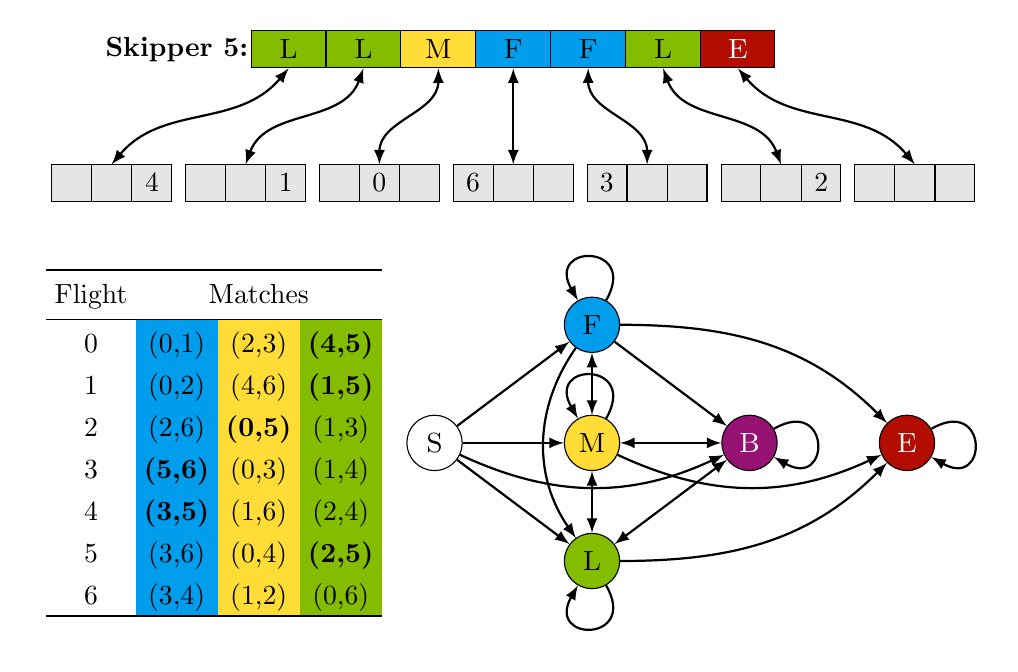
\begin{tikzpicture}
    \begin{scope}[every node/.style={minimum size=2em,inner sep=1}, xshift=-1cm]
        \node (DFAS) [draw, circle, fill=white]                     at (0,  0)   { \textsc{S} };
        \node (DFAF) [draw, circle, fill=uofgcobalt]                at (2,  1.5) { \textsc{F} };
        \node (DFAM) [draw, circle, fill=uofgsunshine]              at (2,  0)   { \textsc{M} };
        \node (DFAL) [draw, circle, fill=uofglawn]                  at (2, -1.5) { \textsc{L} };
        \node (DFAB) [draw, circle, fill=uofgthistle, text=white]   at (4,  0)   { \textsc{B} };
        \node (DFAE) [draw, circle, fill=uofgpillarbox, text=white] at (6,  0)   { \textsc{E} };

        \draw [->, >=latex, thick] (DFAS) to (DFAF);
        \draw [->, >=latex, thick] (DFAS) to (DFAM);
        \draw [->, >=latex, thick] (DFAS) to (DFAL);
        \draw [->, >=latex, thick] (DFAS) to [out=-25, in=-155] (DFAB);

        \draw [->, >=latex, thick] (DFAF) to [out=60, in=120, looseness=6] (DFAF);
        \draw [->, >=latex, thick] (DFAF) to [out=-125, in=125] (DFAL);
        \draw [->, >=latex, thick] (DFAF) to (DFAB);
        \draw [->, >=latex, thick] (DFAF) to [out=0, in=135] (DFAE);

        \draw [<->, >=latex, thick] (DFAF) to (DFAM);

        \draw [->, >=latex, thick] (DFAM) to [out=60, in=120, looseness=6] (DFAM);
        \draw [->, >=latex, thick] (DFAM) to [out=-25, in=-155] (DFAE);

        \draw [<->, >=latex, thick] (DFAM) to (DFAB);
        \draw [<->, >=latex, thick] (DFAM) to (DFAL);

        \draw [->, >=latex, thick] (DFAL) to [out=300, in=240, looseness=6] (DFAL);
        \draw [->, >=latex, thick] (DFAL) to [out=0, in=225] (DFAE);

        \draw [<->, >=latex, thick] (DFAL) to (DFAB);

        \draw [->, >=latex, thick] (DFAB) to [out=30, in=-30, looseness=6] (DFAB);

        \draw [->, >=latex, thick] (DFAE) to [out=30, in=-30, looseness=6] (DFAE);
    \end{scope}

    \begin{scope}[yshift=5cm, scale=0.85]
        \node at (-5, 0) { \textbf{ Skipper 5: } };

        \node (AllArray) [anchor=center, draw, rectangle split, rectangle split horizontal, rectangle split parts=7,
            rectangle split part fill={uofglawn,uofglawn,uofgsunshine,uofgcobalt,uofgcobalt,uofglawn,uofgpillarbox}] at (0, 0) {
            \nodepart[text width=2em, align=center] {one}   \textsc{L}
            \nodepart[text width=2em, align=center] {two}   \textsc{L}
            \nodepart[text width=2em, align=center] {three} \textsc{M}
            \nodepart[text width=2em, align=center] {four}  \textsc{F}
            \nodepart[text width=2em, align=center] {five}  \textsc{F}
            \nodepart[text width=2em, align=center] {six}   \textsc{L}
            \nodepart[text width=2em, align=center, text=white] {seven} \textsc{E}
        };

        \node (Array1) [anchor=center, draw, rectangle split, rectangle split horizontal, rectangle split parts=3,
            rectangle split part fill={black!10!white,black!10!white,black!10!white}]  at (-6, -2) {
            \nodepart[text width=0.75em, align=center] {one}
            \nodepart[text width=0.75em, align=center] {two}
            \nodepart[text width=0.75em, align=center] {three} 4
        };

        \node (Array2) [anchor=center, draw, rectangle split, rectangle split horizontal, rectangle split parts=3,
            rectangle split part fill={black!10!white,black!10!white,black!10!white}]  at (-4, -2) {
            \nodepart[text width=0.75em, align=center] {one}
            \nodepart[text width=0.75em, align=center] {two}
            \nodepart[text width=0.75em, align=center] {three} 1
        };

        \node (Array3) [anchor=center, draw, rectangle split, rectangle split horizontal, rectangle split parts=3,
            rectangle split part fill={black!10!white,black!10!white,black!10!white}]  at (-2, -2) {
            \nodepart[text width=0.75em, align=center] {one}
            \nodepart[text width=0.75em, align=center] {two} 0
            \nodepart[text width=0.75em, align=center] {three}
        };

        \node (Array4) [anchor=center, draw, rectangle split, rectangle split horizontal, rectangle split parts=3,
            rectangle split part fill={black!10!white,black!10!white,black!10!white}]  at (0, -2) {
            \nodepart[text width=0.75em, align=center] {one} 6
            \nodepart[text width=0.75em, align=center] {two}
            \nodepart[text width=0.75em, align=center] {three}
        };

        \node (Array5) [anchor=center, draw, rectangle split, rectangle split horizontal, rectangle split parts=3,
            rectangle split part fill={black!10!white,black!10!white,black!10!white}]  at (2, -2) {
            \nodepart[text width=0.75em, align=center] {one} 3
            \nodepart[text width=0.75em, align=center] {two}
            \nodepart[text width=0.75em, align=center] {three}
        };

        \node (Array6) [anchor=center, draw, rectangle split, rectangle split horizontal, rectangle split parts=3,
            rectangle split part fill={black!10!white,black!10!white,black!10!white}]  at (4, -2) {
            \nodepart[text width=0.75em, align=center] {one}
            \nodepart[text width=0.75em, align=center] {two}
            \nodepart[text width=0.75em, align=center] {three} 2
        };

        \node (Array7) [anchor=center, draw, rectangle split, rectangle split horizontal, rectangle split parts=3,
            rectangle split part fill={black!10!white,black!10!white,black!10!white}]  at (6, -2) {
            \nodepart[text width=0.75em, align=center] {one} \phantom{1}
            \nodepart[text width=0.75em, align=center] {two}
            \nodepart[text width=0.75em, align=center] {three}
        };

        \draw [<->, thick, >=latex] (AllArray.one south) to [in=50, out=230] (Array1.two north);
        \draw [<->, thick, >=latex] (AllArray.two south) to [in=70, out=250] (Array2.two north);
        \draw [<->, thick, >=latex] (AllArray.three south) to [in=90, out=270] (Array3.two north);
        \draw [<->, thick, >=latex] (AllArray.four south) to [in=90, out=270] (Array4.two north);
        \draw [<->, thick, >=latex] (AllArray.five south) to [in=90, out=270] (Array5.two north);
        \draw [<->, thick, >=latex] (AllArray.six south) to [in=110, out=290] (Array6.two north);
        \draw [<->, thick, >=latex] (AllArray.seven south) to [in=130, out=310] (Array7.two north);
    \end{scope}

    \begin{scope}
        \node at (-3.8, 0) {
            \begin{minipage}{4.5cm}
                \centering
                \setlength{\tabcolsep}{3pt}
                \setlength{\aboverulesep}{0pt}
                \setlength{\belowrulesep}{0pt}
                \setlength{\extrarowheight}{.75ex}
                \begin{tabular}{c>{\columncolor{uofgcobalt}}c>{\columncolor{uofgsunshine}}c>{\columncolor{uofglawn}}c}
                    \toprule
                    Flight & \multicolumn{3}{c}{Matches} \\[2pt] \midrule
                    0 & (0,1) & (2,3) & \textbf{(4,5)} \\
                    1 & (0,2) & (4,6) & \textbf{(1,5)} \\
                    2 & (2,6) & \textbf{(0,5)} & (1,3) \\
                    3 & \textbf{(5,6)} & (0,3) & (1,4) \\
                    4 & \textbf{(3,5)} & (1,6) & (2,4) \\
                    5 & (3,6) & (0,4) & \textbf{(2,5)} \\
                    6 & (3,4) & (1,2) & (0,6) \\ \bottomrule
                \end{tabular}
            \end{minipage}
        };
    \end{scope}

    \end{tikzpicture}
    \caption{A pictorial representation of a skipper (skipper 5) with multicoloured state and grey
        timeslots. The schedule for skipper 5 is in bold and the deterministic finite automaton for
        criteria~4, 11 and~12 is drawn with state $\START$ in white, $\FIRST$ in blue, $\MID$ in
        yellow, $\LAST$ in green, $\BYE$ in pink and $\END$ in red.}\label{skipper5}
\end{figure}

\paragraph{Match perspective:} We are now in a position to model criterion~1 (each skipper sails
against every other skipper) and optimisation criterion~10 (minimise boat changes).  In the second
half of Figure~\ref{model:stage1} we present a match perspective of the schedule, using a two
dimensional array of variables $\match$ \eqref{V5}, where $\match[{i,j}]$ is the time slot in which
skippers $\sigma[{i}]$ and $\sigma[{j}]$ meet in a match. Only the half above the diagonal is
represented, and the lower half is made up of exactly the same variables, i.e.\ $\match[{i,j}]$ is
\emph{exactly} the same constrained variable as $\match[{j,i}]$. Constraint \eqref{C6} states that
a match between skippers $\sigma[{i}]$ and $\sigma[{j}]$ takes place at time $k$ (i.e.\
$\match[{i,j}] = k$) if and only if  skipper $\sigma[{i}]$'s $k^{th}$ time slot is skipper
$\sigma[{j}]$ and conversely that skipper $\sigma[{j}]$'s $k^{th}$ time slot is skipper
$\sigma[{i}]$. Variables \eqref{V6} and constraints \eqref{C7} then convert this from time slots to
flights, i.e.\ $\modMatch[{i,j}]$ is the flight in which skippers $\sigma[{i}]$ and $\sigma[{j}]$
meet for a match. Finally, constraint \eqref{C8} ensures that each skipper's match occurs in
different flights. Also, since $\modMatch[{i,j}] \equiv \modMatch[{j,i}]$, setting rows to be all
different also ensures that columns are all different.

\paragraph{Temporal perspective:} We now take a temporal view \eqref{V7}, such that
$\timeVar[{\tau}]$ is a pair $(i,j)$, stating that at time $\tau$ skippers $\sigma[{i}]$ and
$\sigma[{j}]$ are in a match. We channel between the match perspective and the temporal perspective
using \eqref{C9}.

\paragraph{Optimisation criteria:} Finally we have the optimisation criterion (criterion~10) to
minimise the number of boat changes. This is handled by \eqref{V8} and \eqref{C10}.

\paragraph{Decision variables:} The decision variables are $\timeVar[{0}]$ to $\timeVar[{t-1}]$,
i.e.\ for each time slot we decide what match takes place. A symmetry break is made at the top of
search by forcing the first round to contain the matches $(0,1), (2,3), \nldots$, i.e.\ $\forall i
\in \{0 \nldots {m-1}\} : \match[{2i, 2i+1}] = i$. (This is independent of criterion~9, which will
be enforced in a subsequent stage by renumbering.)

\bigskip \noindent Figure~\ref{schedChanges} gives a pictorial view of the entire model, using the 7
skipper and 6 boat problem. On the right we have the 7 skippers with their states and time slots.
Again, on the right we give the schedule actually produced. On the left we have the $\modMatch$ and
$\match$ arrays, and at the bottom the $\timeVar$ array. The arrows show the channeling between
parts of the model.

The schedule presented has 6 boat changes: there are no boat changes in flight 0 (first flight), in
flight 1 skipper 6 has a boat change, in flight 2 skipper 3 has a boat change, in flight 3 skipper
4, in flight 4 skipper 6, in flight 5 skipper 0, and flight 6 skipper 1.

\afterpage{\begin{landscape}
\begin{figure}[p]
    \centering
    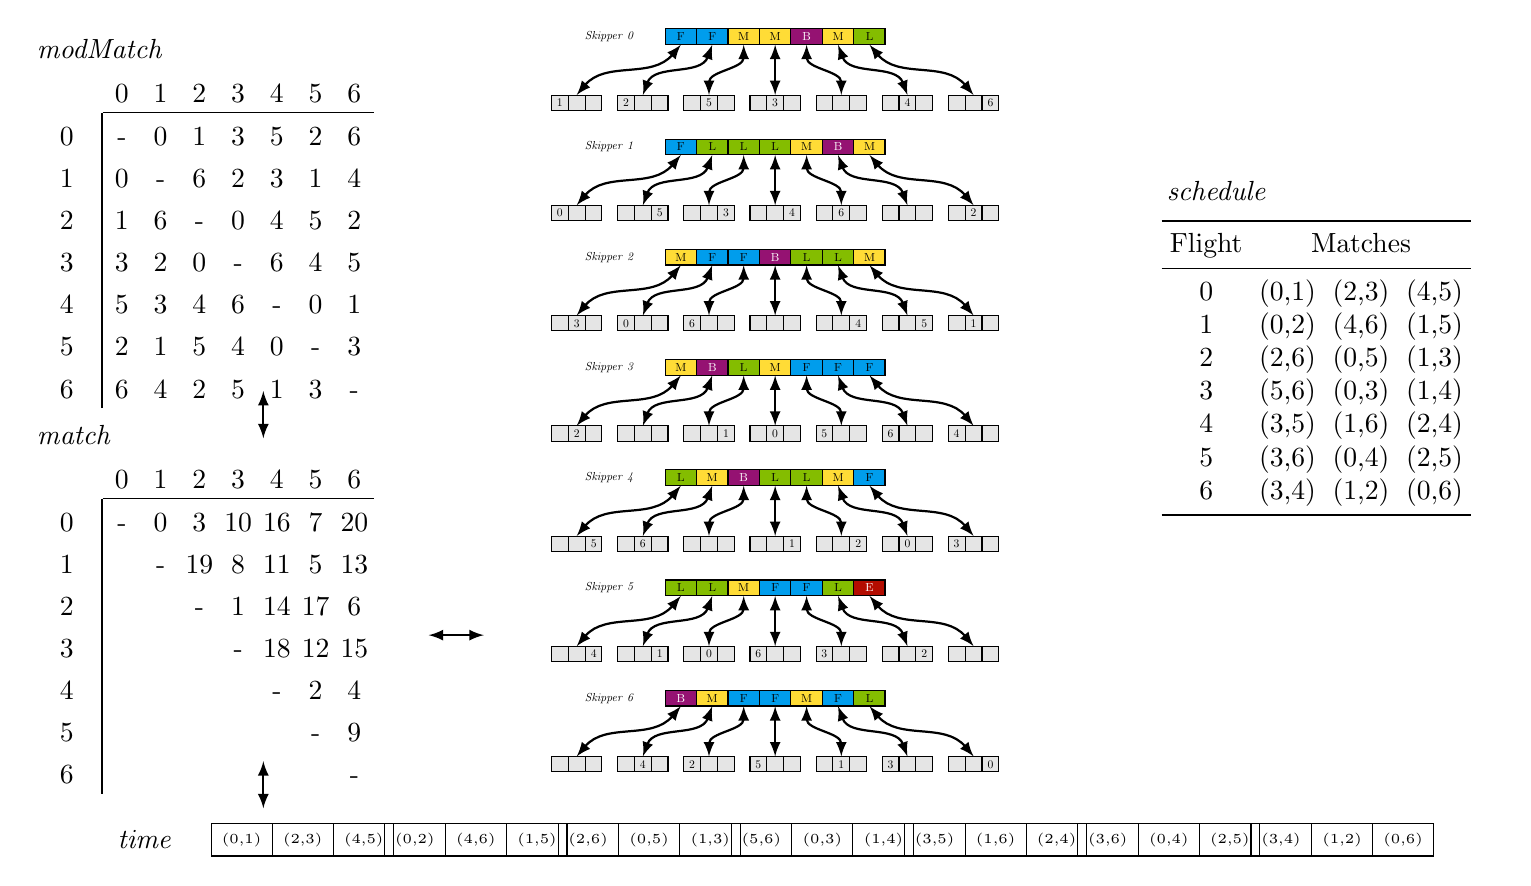
\begin{tikzpicture}
        \begin{scope}
            \node (Time) at (-2, 0) { $\timeVar$ };
            \node (Time0) [font=\tiny, anchor=center, draw, rectangle split, rectangle split horizontal, rectangle split parts=3] at (0, 0) {
                \nodepart[text width=1.5em, align=center] {one}   (0,1)
                \nodepart[text width=1.5em, align=center] {two}   (2,3)
                \nodepart[text width=1.5em, align=center] {three} (4,5)
            };
            \node (Time1) [font=\tiny, anchor=center, draw, rectangle split, rectangle split horizontal, rectangle split parts=3] at (2.2, 0) {
                \nodepart[text width=1.5em, align=center] {one}   (0,2)
                \nodepart[text width=1.5em, align=center] {two}   (4,6)
                \nodepart[text width=1.5em, align=center] {three} (1,5)
            };
            \node (Time2) [font=\tiny, anchor=center, draw, rectangle split, rectangle split horizontal, rectangle split parts=3] at (4.4, 0) {
                \nodepart[text width=1.5em, align=center] {one}   (2,6)
                \nodepart[text width=1.5em, align=center] {two}   (0,5)
                \nodepart[text width=1.5em, align=center] {three} (1,3)
            };
            \node (Time3) [font=\tiny, anchor=center, draw, rectangle split, rectangle split horizontal, rectangle split parts=3] at (6.6, 0) {
                \nodepart[text width=1.5em, align=center] {one}   (5,6)
                \nodepart[text width=1.5em, align=center] {two}   (0,3)
                \nodepart[text width=1.5em, align=center] {three} (1,4)
            };
            \node (Time4) [font=\tiny, anchor=center, draw, rectangle split, rectangle split horizontal, rectangle split parts=3] at (8.8, 0) {
                \nodepart[text width=1.5em, align=center] {one}   (3,5)
                \nodepart[text width=1.5em, align=center] {two}   (1,6)
                \nodepart[text width=1.5em, align=center] {three} (2,4)
            };
            \node (Time5) [font=\tiny, anchor=center, draw, rectangle split, rectangle split horizontal, rectangle split parts=3] at (11.0, 0) {
                \nodepart[text width=1.5em, align=center] {one}   (3,6)
                \nodepart[text width=1.5em, align=center] {two}   (0,4)
                \nodepart[text width=1.5em, align=center] {three} (2,5)
            };
            \node (Time6) [font=\tiny, anchor=center, draw, rectangle split, rectangle split horizontal, rectangle split parts=3] at (13.2, 0) {
                \nodepart[text width=1.5em, align=center] {one}   (3,4)
                \nodepart[text width=1.5em, align=center] {two}   (1,2)
                \nodepart[text width=1.5em, align=center] {three} (0,6)
            };
        \end{scope}

        \begin{scope}[yshift=5cm, xshift=-3.5cm]
            \node [anchor=north west] (MatchTable) at (0, 0) {
                \begin{minipage}{4.5cm}
                    \centering
                    \setlength{\aboverulesep}{0pt}
                    \setlength{\belowrulesep}{0pt}
                    \setlength{\extrarowheight}{.75ex}
                    \setlength{\tabcolsep}{2pt}
                    \begin{tabular}{cccccccc}
                        & 0 & 1 & 2 & 3 & 4 & 5 & 6 \\ \cmidrule{2-8}
                        \multicolumn{1}{l@{\hspace{1em}}|}{0} & ~-~ & 0 & 3 & 10 & 16 & 7 & 20 \\
                        \multicolumn{1}{l@{\hspace{1em}}|}{1} & & ~-~ & 19 & 8 & 11 & 5 & 13 \\
                        \multicolumn{1}{l@{\hspace{1em}}|}{2} & & & ~-~ & 1 & 14 & 17 & 6 \\
                        \multicolumn{1}{l@{\hspace{1em}}|}{3} & & & & ~-~ & 18 & 12 & 15 \\
                        \multicolumn{1}{l@{\hspace{1em}}|}{4} & & & & & ~-~ & 2 & 4 \\
                        \multicolumn{1}{l@{\hspace{1em}}|}{5} & & & & & & ~-~ & 9 \\
                        \multicolumn{1}{l@{\hspace{1em}}|}{6} & & & & & & & ~-~ \\
                    \end{tabular}
                \end{minipage}
            };
            \node [above=-0.1 of MatchTable.north west, anchor=south west] (Match) { $\match$ };
        \end{scope}

        \begin{scope}[yshift=9.9cm, xshift=-3.5cm]
            \node [anchor=north west] (ModMatchTable) at (0, 0) {
                \begin{minipage}{4.5cm}
                    \centering
                    \setlength{\tabcolsep}{2pt}
                    \setlength{\aboverulesep}{0pt}
                    \setlength{\belowrulesep}{0pt}
                    \setlength{\extrarowheight}{.75ex}
                    \begin{tabular}{cccccccc}
                        & 0 & 1 & 2 & 3 & 4 & 5 & 6 \\ \cmidrule{2-8}
                        \multicolumn{1}{l@{\hspace{1em}}|}{0} & ~-~ & 0 & 1 & 3 & 5 & 2 & 6 \\
                        \multicolumn{1}{l@{\hspace{1em}}|}{1} & 0 & ~-~ & 6 & 2 & 3 & 1 & 4 \\
                        \multicolumn{1}{l@{\hspace{1em}}|}{2} & 1 & 6 & ~-~ & 0 & 4 & 5 & 2 \\
                        \multicolumn{1}{l@{\hspace{1em}}|}{3} & 3 & 2 & 0 & ~-~ & 6 & 4 & 5 \\
                        \multicolumn{1}{l@{\hspace{1em}}|}{4} & 5 & 3 & 4 & 6 & ~-~ & 0 & 1 \\
                        \multicolumn{1}{l@{\hspace{1em}}|}{5} & 2 & 1 & 5 & 4 & 0 & ~-~ & 3 \\
                        \multicolumn{1}{l@{\hspace{1em}}|}{6} & 6 & 4 & 2 & 5 & 1 & 3 & ~-~ \\
                    \end{tabular}
                \end{minipage}
            };
            \node [above=-0.1 of ModMatchTable.north west, anchor=south west] (ModMatch) { $\modMatch$ };
        \end{scope}

        \begin{scope}[yshift=10.2cm, xshift=6cm, scale=0.42, every node/.style={transform shape}]
            \node at (-5, 0) { $\mathit{Skipper~0}$ };

            \node (AllArray) [anchor=center, draw, rectangle split, rectangle split horizontal, rectangle split parts=7,
            rectangle split part fill={uofgcobalt,uofgcobalt,uofgsunshine,uofgsunshine,uofgthistle,uofgsunshine,uofglawn}] at (0, 0) {
                \nodepart[text width=2em, align=center] {one}   \textsc{F}
                \nodepart[text width=2em, align=center] {two}   \textsc{F}
                \nodepart[text width=2em, align=center] {three} \textsc{M}
                \nodepart[text width=2em, align=center] {four}  \textsc{M}
                \nodepart[text width=2em, align=center, text=white] {five} \textsc{B}
                \nodepart[text width=2em, align=center] {six}   \textsc{M}
                \nodepart[text width=2em, align=center] {seven} \textsc{L}
            };

            \node (Array1) [anchor=center, draw, rectangle split, rectangle split horizontal, rectangle split parts=3,
                rectangle split part fill={black!10!white,black!10!white,black!10!white}]  at (-6, -2) {
                \nodepart[text width=0.75em, align=center] {one} 1
                \nodepart[text width=0.75em, align=center] {two}
                \nodepart[text width=0.75em, align=center] {three}
            };

            \node (Array2) [anchor=center, draw, rectangle split, rectangle split horizontal, rectangle split parts=3,
                rectangle split part fill={black!10!white,black!10!white,black!10!white}]  at (-4, -2) {
                \nodepart[text width=0.75em, align=center] {one} 2
                \nodepart[text width=0.75em, align=center] {two}
                \nodepart[text width=0.75em, align=center] {three}
            };

            \node (Array3) [anchor=center, draw, rectangle split, rectangle split horizontal, rectangle split parts=3,
                rectangle split part fill={black!10!white,black!10!white,black!10!white}]  at (-2, -2) {
                \nodepart[text width=0.75em, align=center] {one}
                \nodepart[text width=0.75em, align=center] {two} 5
                \nodepart[text width=0.75em, align=center] {three}
            };

            \node (Array4) [anchor=center, draw, rectangle split, rectangle split horizontal, rectangle split parts=3,
                rectangle split part fill={black!10!white,black!10!white,black!10!white}]  at (0, -2) {
                \nodepart[text width=0.75em, align=center] {one}
                \nodepart[text width=0.75em, align=center] {two} 3
                \nodepart[text width=0.75em, align=center] {three}
            };

            \node (Array5) [anchor=center, draw, rectangle split, rectangle split horizontal, rectangle split parts=3,
                rectangle split part fill={black!10!white,black!10!white,black!10!white}]  at (2, -2) {
                \nodepart[text width=0.75em, align=center] {one} \phantom{1}
                \nodepart[text width=0.75em, align=center] {two}
                \nodepart[text width=0.75em, align=center] {three}
            };

            \node (Array6) [anchor=center, draw, rectangle split, rectangle split horizontal, rectangle split parts=3,
                rectangle split part fill={black!10!white,black!10!white,black!10!white}]  at (4, -2) {
                \nodepart[text width=0.75em, align=center] {one}
                \nodepart[text width=0.75em, align=center] {two} 4
                \nodepart[text width=0.75em, align=center] {three}
            };

            \node (Array7) [anchor=center, draw, rectangle split, rectangle split horizontal, rectangle split parts=3,
                rectangle split part fill={black!10!white,black!10!white,black!10!white}]  at (6, -2) {
                \nodepart[text width=0.75em, align=center] {one}
                \nodepart[text width=0.75em, align=center] {two}
                \nodepart[text width=0.75em, align=center] {three} 6
            };

            \draw [<->, thick, >=latex] (AllArray.one south) to [in=50, out=230] (Array1.two north);
            \draw [<->, thick, >=latex] (AllArray.two south) to [in=70, out=250] (Array2.two north);
            \draw [<->, thick, >=latex] (AllArray.three south) to [in=90, out=270] (Array3.two north);
            \draw [<->, thick, >=latex] (AllArray.four south) to [in=90, out=270] (Array4.two north);
            \draw [<->, thick, >=latex] (AllArray.five south) to [in=90, out=270] (Array5.two north);
            \draw [<->, thick, >=latex] (AllArray.six south) to [in=110, out=290] (Array6.two north);
            \draw [<->, thick, >=latex] (AllArray.seven south) to [in=130, out=310] (Array7.two north);
        \end{scope}

        \begin{scope}[yshift=8.8cm, xshift=6cm, scale=0.42, every node/.style={transform shape}]
            \node at (-5, 0) { $\mathit{Skipper~1}$ };

            \node (AllArray) [anchor=center, draw, rectangle split, rectangle split horizontal, rectangle split parts=7,
            rectangle split part fill={uofgcobalt,uofglawn,uofglawn,uofglawn,uofgsunshine,uofgthistle,uofgsunshine}] at (0, 0) {
                \nodepart[text width=2em, align=center] {one}   \textsc{F}
                \nodepart[text width=2em, align=center] {two}   \textsc{L}
                \nodepart[text width=2em, align=center] {three} \textsc{L}
                \nodepart[text width=2em, align=center] {four}  \textsc{L}
                \nodepart[text width=2em, align=center] {five}  \textsc{M}
                \nodepart[text width=2em, align=center, text=white] {six}   \textsc{B}
                \nodepart[text width=2em, align=center] {seven} \textsc{M}
            };

            \node (Array1) [anchor=center, draw, rectangle split, rectangle split horizontal, rectangle split parts=3,
                rectangle split part fill={black!10!white,black!10!white,black!10!white}]  at (-6, -2) {
                \nodepart[text width=0.75em, align=center] {one} 0
                \nodepart[text width=0.75em, align=center] {two}
                \nodepart[text width=0.75em, align=center] {three}
            };

            \node (Array2) [anchor=center, draw, rectangle split, rectangle split horizontal, rectangle split parts=3,
                rectangle split part fill={black!10!white,black!10!white,black!10!white}]  at (-4, -2) {
                \nodepart[text width=0.75em, align=center] {one}
                \nodepart[text width=0.75em, align=center] {two}
                \nodepart[text width=0.75em, align=center] {three} 5
            };

            \node (Array3) [anchor=center, draw, rectangle split, rectangle split horizontal, rectangle split parts=3,
                rectangle split part fill={black!10!white,black!10!white,black!10!white}]  at (-2, -2) {
                \nodepart[text width=0.75em, align=center] {one}
                \nodepart[text width=0.75em, align=center] {two}
                \nodepart[text width=0.75em, align=center] {three} 3
            };

            \node (Array4) [anchor=center, draw, rectangle split, rectangle split horizontal, rectangle split parts=3,
                rectangle split part fill={black!10!white,black!10!white,black!10!white}]  at (0, -2) {
                \nodepart[text width=0.75em, align=center] {one}
                \nodepart[text width=0.75em, align=center] {two}
                \nodepart[text width=0.75em, align=center] {three} 4
            };

            \node (Array5) [anchor=center, draw, rectangle split, rectangle split horizontal, rectangle split parts=3,
                rectangle split part fill={black!10!white,black!10!white,black!10!white}]  at (2, -2) {
                \nodepart[text width=0.75em, align=center] {one}
                \nodepart[text width=0.75em, align=center] {two} 6
                \nodepart[text width=0.75em, align=center] {three}
            };

            \node (Array6) [anchor=center, draw, rectangle split, rectangle split horizontal, rectangle split parts=3,
                rectangle split part fill={black!10!white,black!10!white,black!10!white}]  at (4, -2) {
                \nodepart[text width=0.75em, align=center] {one} \phantom{1}
                \nodepart[text width=0.75em, align=center] {two}
                \nodepart[text width=0.75em, align=center] {three}
            };

            \node (Array7) [anchor=center, draw, rectangle split, rectangle split horizontal, rectangle split parts=3,
                rectangle split part fill={black!10!white,black!10!white,black!10!white}]  at (6, -2) {
                \nodepart[text width=0.75em, align=center] {one}
                \nodepart[text width=0.75em, align=center] {two} 2
                \nodepart[text width=0.75em, align=center] {three}
            };

            \draw [<->, thick, >=latex] (AllArray.one south) to [in=50, out=230] (Array1.two north);
            \draw [<->, thick, >=latex] (AllArray.two south) to [in=70, out=250] (Array2.two north);
            \draw [<->, thick, >=latex] (AllArray.three south) to [in=90, out=270] (Array3.two north);
            \draw [<->, thick, >=latex] (AllArray.four south) to [in=90, out=270] (Array4.two north);
            \draw [<->, thick, >=latex] (AllArray.five south) to [in=90, out=270] (Array5.two north);
            \draw [<->, thick, >=latex] (AllArray.six south) to [in=110, out=290] (Array6.two north);
            \draw [<->, thick, >=latex] (AllArray.seven south) to [in=130, out=310] (Array7.two north);
        \end{scope}

        \begin{scope}[yshift=7.4cm, xshift=6cm, scale=0.42, every node/.style={transform shape}]
            \node at (-5, 0) { $\mathit{Skipper~2}$ };

            \node (AllArray) [anchor=center, draw, rectangle split, rectangle split horizontal, rectangle split parts=7,
            rectangle split part fill={uofgsunshine,uofgcobalt,uofgcobalt,uofgthistle,uofglawn,uofglawn,uofgsunshine}] at (0, 0) {
                \nodepart[text width=2em, align=center] {one}   \textsc{M}
                \nodepart[text width=2em, align=center] {two}   \textsc{F}
                \nodepart[text width=2em, align=center] {three} \textsc{F}
                \nodepart[text width=2em, align=center, text=white] {four}  \textsc{B}
                \nodepart[text width=2em, align=center] {five}  \textsc{L}
                \nodepart[text width=2em, align=center] {six}   \textsc{L}
                \nodepart[text width=2em, align=center] {seven} \textsc{M}
            };

            \node (Array1) [anchor=center, draw, rectangle split, rectangle split horizontal, rectangle split parts=3,
                rectangle split part fill={black!10!white,black!10!white,black!10!white}]  at (-6, -2) {
                \nodepart[text width=0.75em, align=center] {one}
                \nodepart[text width=0.75em, align=center] {two} 3
                \nodepart[text width=0.75em, align=center] {three}
            };

            \node (Array2) [anchor=center, draw, rectangle split, rectangle split horizontal, rectangle split parts=3,
                rectangle split part fill={black!10!white,black!10!white,black!10!white}]  at (-4, -2) {
                \nodepart[text width=0.75em, align=center] {one} 0
                \nodepart[text width=0.75em, align=center] {two}
                \nodepart[text width=0.75em, align=center] {three}
            };

            \node (Array3) [anchor=center, draw, rectangle split, rectangle split horizontal, rectangle split parts=3,
                rectangle split part fill={black!10!white,black!10!white,black!10!white}]  at (-2, -2) {
                \nodepart[text width=0.75em, align=center] {one} 6
                \nodepart[text width=0.75em, align=center] {two}
                \nodepart[text width=0.75em, align=center] {three}
            };

            \node (Array4) [anchor=center, draw, rectangle split, rectangle split horizontal, rectangle split parts=3,
                rectangle split part fill={black!10!white,black!10!white,black!10!white}]  at (0, -2) {
                \nodepart[text width=0.75em, align=center] {one} \phantom{1}
                \nodepart[text width=0.75em, align=center] {two}
                \nodepart[text width=0.75em, align=center] {three}
            };

            \node (Array5) [anchor=center, draw, rectangle split, rectangle split horizontal, rectangle split parts=3,
                rectangle split part fill={black!10!white,black!10!white,black!10!white}]  at (2, -2) {
                \nodepart[text width=0.75em, align=center] {one}
                \nodepart[text width=0.75em, align=center] {two}
                \nodepart[text width=0.75em, align=center] {three} 4
            };

            \node (Array6) [anchor=center, draw, rectangle split, rectangle split horizontal, rectangle split parts=3,
                rectangle split part fill={black!10!white,black!10!white,black!10!white}]  at (4, -2) {
                \nodepart[text width=0.75em, align=center] {one}
                \nodepart[text width=0.75em, align=center] {two}
                \nodepart[text width=0.75em, align=center] {three} 5
            };

            \node (Array7) [anchor=center, draw, rectangle split, rectangle split horizontal, rectangle split parts=3,
                rectangle split part fill={black!10!white,black!10!white,black!10!white}]  at (6, -2) {
                \nodepart[text width=0.75em, align=center] {one}
                \nodepart[text width=0.75em, align=center] {two} 1
                \nodepart[text width=0.75em, align=center] {three}
            };

            \draw [<->, thick, >=latex] (AllArray.one south) to [in=50, out=230] (Array1.two north);
            \draw [<->, thick, >=latex] (AllArray.two south) to [in=70, out=250] (Array2.two north);
            \draw [<->, thick, >=latex] (AllArray.three south) to [in=90, out=270] (Array3.two north);
            \draw [<->, thick, >=latex] (AllArray.four south) to [in=90, out=270] (Array4.two north);
            \draw [<->, thick, >=latex] (AllArray.five south) to [in=90, out=270] (Array5.two north);
            \draw [<->, thick, >=latex] (AllArray.six south) to [in=110, out=290] (Array6.two north);
            \draw [<->, thick, >=latex] (AllArray.seven south) to [in=130, out=310] (Array7.two north);
        \end{scope}

        \begin{scope}[yshift=6.0cm, xshift=6cm, scale=0.42, every node/.style={transform shape}]
            \node at (-5, 0) { $\mathit{Skipper~3}$ };

            \node (AllArray) [anchor=center, draw, rectangle split, rectangle split horizontal, rectangle split parts=7,
            rectangle split part fill={uofgsunshine,uofgthistle,uofglawn,uofgsunshine,uofgcobalt,uofgcobalt,uofgcobalt}] at (0, 0) {
                \nodepart[text width=2em, align=center] {one}   \textsc{M}
                \nodepart[text width=2em, align=center, text=white] {two}   \textsc{B}
                \nodepart[text width=2em, align=center] {three} \textsc{L}
                \nodepart[text width=2em, align=center] {four}  \textsc{M}
                \nodepart[text width=2em, align=center] {five}  \textsc{F}
                \nodepart[text width=2em, align=center] {six}   \textsc{F}
                \nodepart[text width=2em, align=center] {seven} \textsc{F}
            };

            \node (Array1) [anchor=center, draw, rectangle split, rectangle split horizontal, rectangle split parts=3,
                rectangle split part fill={black!10!white,black!10!white,black!10!white}]  at (-6, -2) {
                \nodepart[text width=0.75em, align=center] {one}
                \nodepart[text width=0.75em, align=center] {two} 2
                \nodepart[text width=0.75em, align=center] {three}
            };

            \node (Array2) [anchor=center, draw, rectangle split, rectangle split horizontal, rectangle split parts=3,
                rectangle split part fill={black!10!white,black!10!white,black!10!white}]  at (-4, -2) {
                \nodepart[text width=0.75em, align=center] {one} \phantom{1}
                \nodepart[text width=0.75em, align=center] {two}
                \nodepart[text width=0.75em, align=center] {three}
            };

            \node (Array3) [anchor=center, draw, rectangle split, rectangle split horizontal, rectangle split parts=3,
                rectangle split part fill={black!10!white,black!10!white,black!10!white}]  at (-2, -2) {
                \nodepart[text width=0.75em, align=center] {one}
                \nodepart[text width=0.75em, align=center] {two}
                \nodepart[text width=0.75em, align=center] {three} 1
            };

            \node (Array4) [anchor=center, draw, rectangle split, rectangle split horizontal, rectangle split parts=3,
                rectangle split part fill={black!10!white,black!10!white,black!10!white}]  at (0, -2) {
                \nodepart[text width=0.75em, align=center] {one}
                \nodepart[text width=0.75em, align=center] {two} 0
                \nodepart[text width=0.75em, align=center] {three}
            };

            \node (Array5) [anchor=center, draw, rectangle split, rectangle split horizontal, rectangle split parts=3,
                rectangle split part fill={black!10!white,black!10!white,black!10!white}]  at (2, -2) {
                \nodepart[text width=0.75em, align=center] {one} 5
                \nodepart[text width=0.75em, align=center] {two}
                \nodepart[text width=0.75em, align=center] {three}
            };

            \node (Array6) [anchor=center, draw, rectangle split, rectangle split horizontal, rectangle split parts=3,
                rectangle split part fill={black!10!white,black!10!white,black!10!white}]  at (4, -2) {
                \nodepart[text width=0.75em, align=center] {one} 6
                \nodepart[text width=0.75em, align=center] {two}
                \nodepart[text width=0.75em, align=center] {three}
            };

            \node (Array7) [anchor=center, draw, rectangle split, rectangle split horizontal, rectangle split parts=3,
                rectangle split part fill={black!10!white,black!10!white,black!10!white}]  at (6, -2) {
                \nodepart[text width=0.75em, align=center] {one} 4
                \nodepart[text width=0.75em, align=center] {two}
                \nodepart[text width=0.75em, align=center] {three}
            };

            \draw [<->, thick, >=latex] (AllArray.one south) to [in=50, out=230] (Array1.two north);
            \draw [<->, thick, >=latex] (AllArray.two south) to [in=70, out=250] (Array2.two north);
            \draw [<->, thick, >=latex] (AllArray.three south) to [in=90, out=270] (Array3.two north);
            \draw [<->, thick, >=latex] (AllArray.four south) to [in=90, out=270] (Array4.two north);
            \draw [<->, thick, >=latex] (AllArray.five south) to [in=90, out=270] (Array5.two north);
            \draw [<->, thick, >=latex] (AllArray.six south) to [in=110, out=290] (Array6.two north);
            \draw [<->, thick, >=latex] (AllArray.seven south) to [in=130, out=310] (Array7.two north);
        \end{scope}

        \begin{scope}[yshift=4.6cm, xshift=6cm, scale=0.42, every node/.style={transform shape}]
            \node at (-5, 0) { $\mathit{Skipper~4}$ };

            \node (AllArray) [anchor=center, draw, rectangle split, rectangle split horizontal, rectangle split parts=7,
            rectangle split part fill={uofglawn,uofgsunshine,uofgthistle,uofglawn,uofglawn,uofgsunshine,uofgcobalt}] at (0, 0) {
                \nodepart[text width=2em, align=center] {one}   \textsc{L}
                \nodepart[text width=2em, align=center] {two}   \textsc{M}
                \nodepart[text width=2em, align=center, text=white] {three} \textsc{B}
                \nodepart[text width=2em, align=center] {four}  \textsc{L}
                \nodepart[text width=2em, align=center] {five}  \textsc{L}
                \nodepart[text width=2em, align=center] {six}   \textsc{M}
                \nodepart[text width=2em, align=center] {seven} \textsc{F}
            };

            \node (Array1) [anchor=center, draw, rectangle split, rectangle split horizontal, rectangle split parts=3,
                rectangle split part fill={black!10!white,black!10!white,black!10!white}]  at (-6, -2) {
                \nodepart[text width=0.75em, align=center] {one}
                \nodepart[text width=0.75em, align=center] {two}
                \nodepart[text width=0.75em, align=center] {three} 5
            };

            \node (Array2) [anchor=center, draw, rectangle split, rectangle split horizontal, rectangle split parts=3,
                rectangle split part fill={black!10!white,black!10!white,black!10!white}]  at (-4, -2) {
                \nodepart[text width=0.75em, align=center] {one}
                \nodepart[text width=0.75em, align=center] {two} 6
                \nodepart[text width=0.75em, align=center] {three}
            };

            \node (Array3) [anchor=center, draw, rectangle split, rectangle split horizontal, rectangle split parts=3,
                rectangle split part fill={black!10!white,black!10!white,black!10!white}]  at (-2, -2) {
                \nodepart[text width=0.75em, align=center] {one} \phantom{1}
                \nodepart[text width=0.75em, align=center] {two}
                \nodepart[text width=0.75em, align=center] {three}
            };

            \node (Array4) [anchor=center, draw, rectangle split, rectangle split horizontal, rectangle split parts=3,
                rectangle split part fill={black!10!white,black!10!white,black!10!white}]  at (0, -2) {
                \nodepart[text width=0.75em, align=center] {one}
                \nodepart[text width=0.75em, align=center] {two}
                \nodepart[text width=0.75em, align=center] {three} 1
            };

            \node (Array5) [anchor=center, draw, rectangle split, rectangle split horizontal, rectangle split parts=3,
                rectangle split part fill={black!10!white,black!10!white,black!10!white}]  at (2, -2) {
                \nodepart[text width=0.75em, align=center] {one}
                \nodepart[text width=0.75em, align=center] {two}
                \nodepart[text width=0.75em, align=center] {three} 2
            };

            \node (Array6) [anchor=center, draw, rectangle split, rectangle split horizontal, rectangle split parts=3,
                rectangle split part fill={black!10!white,black!10!white,black!10!white}]  at (4, -2) {
                \nodepart[text width=0.75em, align=center] {one}
                \nodepart[text width=0.75em, align=center] {two} 0
                \nodepart[text width=0.75em, align=center] {three}
            };

            \node (Array7) [anchor=center, draw, rectangle split, rectangle split horizontal, rectangle split parts=3,
                rectangle split part fill={black!10!white,black!10!white,black!10!white}]  at (6, -2) {
                \nodepart[text width=0.75em, align=center] {one} 3
                \nodepart[text width=0.75em, align=center] {two}
                \nodepart[text width=0.75em, align=center] {three}
            };

            \draw [<->, thick, >=latex] (AllArray.one south) to [in=50, out=230] (Array1.two north);
            \draw [<->, thick, >=latex] (AllArray.two south) to [in=70, out=250] (Array2.two north);
            \draw [<->, thick, >=latex] (AllArray.three south) to [in=90, out=270] (Array3.two north);
            \draw [<->, thick, >=latex] (AllArray.four south) to [in=90, out=270] (Array4.two north);
            \draw [<->, thick, >=latex] (AllArray.five south) to [in=90, out=270] (Array5.two north);
            \draw [<->, thick, >=latex] (AllArray.six south) to [in=110, out=290] (Array6.two north);
            \draw [<->, thick, >=latex] (AllArray.seven south) to [in=130, out=310] (Array7.two north);
        \end{scope}

        \begin{scope}[yshift=3.2cm, xshift=6cm, scale=0.42, every node/.style={transform shape}]
            \node at (-5, 0) { $\mathit{Skipper~5}$ };

            \node (AllArray) [anchor=center, draw, rectangle split, rectangle split horizontal, rectangle split parts=7,
            rectangle split part fill={uofglawn,uofglawn,uofgsunshine,uofgcobalt,uofgcobalt,uofglawn,uofgpillarbox}] at (0, 0) {
                \nodepart[text width=2em, align=center] {one}   \textsc{L}
                \nodepart[text width=2em, align=center] {two}   \textsc{L}
                \nodepart[text width=2em, align=center] {three} \textsc{M}
                \nodepart[text width=2em, align=center] {four}  \textsc{F}
                \nodepart[text width=2em, align=center] {five}  \textsc{F}
                \nodepart[text width=2em, align=center] {six}   \textsc{L}
                \nodepart[text width=2em, align=center, text=white] {seven} \textsc{E}
            };

            \node (Array1) [anchor=center, draw, rectangle split, rectangle split horizontal, rectangle split parts=3,
                rectangle split part fill={black!10!white,black!10!white,black!10!white}]  at (-6, -2) {
                \nodepart[text width=0.75em, align=center] {one}
                \nodepart[text width=0.75em, align=center] {two}
                \nodepart[text width=0.75em, align=center] {three} 4
            };

            \node (Array2) [anchor=center, draw, rectangle split, rectangle split horizontal, rectangle split parts=3,
                rectangle split part fill={black!10!white,black!10!white,black!10!white}]  at (-4, -2) {
                \nodepart[text width=0.75em, align=center] {one}
                \nodepart[text width=0.75em, align=center] {two}
                \nodepart[text width=0.75em, align=center] {three} 1
            };

            \node (Array3) [anchor=center, draw, rectangle split, rectangle split horizontal, rectangle split parts=3,
                rectangle split part fill={black!10!white,black!10!white,black!10!white}]  at (-2, -2) {
                \nodepart[text width=0.75em, align=center] {one}
                \nodepart[text width=0.75em, align=center] {two} 0
                \nodepart[text width=0.75em, align=center] {three}
            };

            \node (Array4) [anchor=center, draw, rectangle split, rectangle split horizontal, rectangle split parts=3,
                rectangle split part fill={black!10!white,black!10!white,black!10!white}]  at (0, -2) {
                \nodepart[text width=0.75em, align=center] {one} 6
                \nodepart[text width=0.75em, align=center] {two}
                \nodepart[text width=0.75em, align=center] {three}
            };

            \node (Array5) [anchor=center, draw, rectangle split, rectangle split horizontal, rectangle split parts=3,
                rectangle split part fill={black!10!white,black!10!white,black!10!white}]  at (2, -2) {
                \nodepart[text width=0.75em, align=center] {one} 3
                \nodepart[text width=0.75em, align=center] {two}
                \nodepart[text width=0.75em, align=center] {three}
            };

            \node (Array6) [anchor=center, draw, rectangle split, rectangle split horizontal, rectangle split parts=3,
                rectangle split part fill={black!10!white,black!10!white,black!10!white}]  at (4, -2) {
                \nodepart[text width=0.75em, align=center] {one}
                \nodepart[text width=0.75em, align=center] {two}
                \nodepart[text width=0.75em, align=center] {three} 2
            };

            \node (Array7) [anchor=center, draw, rectangle split, rectangle split horizontal, rectangle split parts=3,
                rectangle split part fill={black!10!white,black!10!white,black!10!white}]  at (6, -2) {
                \nodepart[text width=0.75em, align=center] {one} \phantom{1}
                \nodepart[text width=0.75em, align=center] {two}
                \nodepart[text width=0.75em, align=center] {three}
            };

            \draw [<->, thick, >=latex] (AllArray.one south) to [in=50, out=230] (Array1.two north);
            \draw [<->, thick, >=latex] (AllArray.two south) to [in=70, out=250] (Array2.two north);
            \draw [<->, thick, >=latex] (AllArray.three south) to [in=90, out=270] (Array3.two north);
            \draw [<->, thick, >=latex] (AllArray.four south) to [in=90, out=270] (Array4.two north);
            \draw [<->, thick, >=latex] (AllArray.five south) to [in=90, out=270] (Array5.two north);
            \draw [<->, thick, >=latex] (AllArray.six south) to [in=110, out=290] (Array6.two north);
            \draw [<->, thick, >=latex] (AllArray.seven south) to [in=130, out=310] (Array7.two north);
        \end{scope}

        \begin{scope}[yshift=1.8cm, xshift=6cm, scale=0.42, every node/.style={transform shape}]
            \node at (-5, 0) { $\mathit{Skipper~6}$ };

            \node (AllArray) [anchor=center, draw, rectangle split, rectangle split horizontal, rectangle split parts=7,
            rectangle split part fill={uofgthistle,uofgsunshine,uofgcobalt,uofgcobalt,uofgsunshine,uofgcobalt,uofglawn}] at (0, 0) {
                \nodepart[text width=2em, align=center, text=white] {one}   \textsc{B}
                \nodepart[text width=2em, align=center] {two}   \textsc{M}
                \nodepart[text width=2em, align=center] {three} \textsc{F}
                \nodepart[text width=2em, align=center] {four}  \textsc{F}
                \nodepart[text width=2em, align=center] {five}  \textsc{M}
                \nodepart[text width=2em, align=center] {six}   \textsc{F}
                \nodepart[text width=2em, align=center] {seven} \textsc{L}
            };

            \node (Array1) [anchor=center, draw, rectangle split, rectangle split horizontal, rectangle split parts=3,
                rectangle split part fill={black!10!white,black!10!white,black!10!white}]  at (-6, -2) {
                \nodepart[text width=0.75em, align=center] {one} \phantom{1}
                \nodepart[text width=0.75em, align=center] {two}
                \nodepart[text width=0.75em, align=center] {three}
            };

            \node (Array2) [anchor=center, draw, rectangle split, rectangle split horizontal, rectangle split parts=3,
                rectangle split part fill={black!10!white,black!10!white,black!10!white}]  at (-4, -2) {
                \nodepart[text width=0.75em, align=center] {one}
                \nodepart[text width=0.75em, align=center] {two} 4
                \nodepart[text width=0.75em, align=center] {three}
            };

            \node (Array3) [anchor=center, draw, rectangle split, rectangle split horizontal, rectangle split parts=3,
                rectangle split part fill={black!10!white,black!10!white,black!10!white}]  at (-2, -2) {
                \nodepart[text width=0.75em, align=center] {one} 2
                \nodepart[text width=0.75em, align=center] {two}
                \nodepart[text width=0.75em, align=center] {three}
            };

            \node (Array4) [anchor=center, draw, rectangle split, rectangle split horizontal, rectangle split parts=3,
                rectangle split part fill={black!10!white,black!10!white,black!10!white}]  at (0, -2) {
                \nodepart[text width=0.75em, align=center] {one} 5
                \nodepart[text width=0.75em, align=center] {two}
                \nodepart[text width=0.75em, align=center] {three}
            };

            \node (Array5) [anchor=center, draw, rectangle split, rectangle split horizontal, rectangle split parts=3,
                rectangle split part fill={black!10!white,black!10!white,black!10!white}]  at (2, -2) {
                \nodepart[text width=0.75em, align=center] {one}
                \nodepart[text width=0.75em, align=center] {two} 1
                \nodepart[text width=0.75em, align=center] {three}
            };

            \node (Array6) [anchor=center, draw, rectangle split, rectangle split horizontal, rectangle split parts=3,
                rectangle split part fill={black!10!white,black!10!white,black!10!white}]  at (4, -2) {
                \nodepart[text width=0.75em, align=center] {one} 3
                \nodepart[text width=0.75em, align=center] {two}
                \nodepart[text width=0.75em, align=center] {three}
            };

            \node (Array7) [anchor=center, draw, rectangle split, rectangle split horizontal, rectangle split parts=3,
                rectangle split part fill={black!10!white,black!10!white,black!10!white}]  at (6, -2) {
                \nodepart[text width=0.75em, align=center] {one}
                \nodepart[text width=0.75em, align=center] {two}
                \nodepart[text width=0.75em, align=center] {three} 0
            };

            \draw [<->, thick, >=latex] (AllArray.one south) to [in=50, out=230] (Array1.two north);
            \draw [<->, thick, >=latex] (AllArray.two south) to [in=70, out=250] (Array2.two north);
            \draw [<->, thick, >=latex] (AllArray.three south) to [in=90, out=270] (Array3.two north);
            \draw [<->, thick, >=latex] (AllArray.four south) to [in=90, out=270] (Array4.two north);
            \draw [<->, thick, >=latex] (AllArray.five south) to [in=90, out=270] (Array5.two north);
            \draw [<->, thick, >=latex] (AllArray.six south) to [in=110, out=290] (Array6.two north);
            \draw [<->, thick, >=latex] (AllArray.seven south) to [in=130, out=310] (Array7.two north);
        \end{scope}

        \begin{scope}
            \node [anchor=north west] (Schedule) at (10.5, 8) {
                \begin{minipage}{4.5cm}
                    \centering
                    \setlength{\tabcolsep}{3pt}
                    \begin{tabular}{cccc}
                        \toprule
                        Flight & \multicolumn{3}{c}{Matches} \\ \midrule
                        0 & (0,1) & (2,3) & (4,5) \\
                        1 & (0,2) & (4,6) & (1,5) \\
                        2 & (2,6) & (0,5) & (1,3) \\
                        3 & (5,6) & (0,3) & (1,4) \\
                        4 & (3,5) & (1,6) & (2,4) \\
                        5 & (3,6) & (0,4) & (2,5) \\
                        6 & (3,4) & (1,2) & (0,6) \\ \bottomrule
                    \end{tabular}
                \end{minipage}
            };
            \node [above=0 of Schedule.north west, anchor=south west] (Match) { \hspace*{1em}$\mathit{schedule}$ };
        \end{scope}

        \begin{scope}
            \draw [<->, thick, >=latex] (-0.5, 5.1) to (-0.5, 5.7);
            \draw [<->, thick, >=latex] (-0.5, 0.4) to (-0.5, 1.0);
            \draw [<->, thick, >=latex] (1.6, 2.6) to (2.3, 2.6);
        \end{scope}

    \end{tikzpicture}
    \caption{A pictorial representation of the entire model of the schedule for 7 skippers and 6 boats.
        The schedule is reproduced on the right. In the centre we have the 7 skippers, on left the
        $\modMatch$ and $\match$ arrays, and along the bottom the $\timeVar$
    array. The arrows signify channeling between parts of the model.}
    \label{schedChanges}
\end{figure}
\end{landscape}

\begin{figure}[p]
\setlength{\mathindent}{1em}
\setlength{\abovedisplayskip}{0pt}
\setlength{\belowdisplayskip}{0pt}
\setlength{\abovecaptionskip}{0pt}
\begin{framed}
\begin{align}
    \intertext{The objective value from stage 1 is used as a hard constraint:\smallskip}
    & \totalBoatChanges \leq \beta \tag{C11} \label{C11}
\end{align}
\end{framed}\begin{framed}
\begin{align}
    \intertext{A copy of these variables and constraints is created for each skipper $\sigma$:\smallskip}
    & \forall i \in \{ 0 \nldots m{-}1 \} : \forall j \in \{ 0 \nldots f{-}1 \} : \nonumber \\
    & \hspace*{1em} \position[{i,j}] \in \{0,1\} \tag{V9} \label{V9} \\
    & \hspace*{1em} \position[{i,j}] = 1 \Leftrightarrow \timeSlot[{m.j+i}] \geq 0 \tag{C12} \label{C12} \\
    & \forall i \in \{ 0 \nldots m{-}1 \} : \nonumber \\
    & \hspace*{1em} \imbalance[{i}] \in \mathbb{N} \label{V10} \tag{V10} \\
    & \hspace*{1em} \imbalance[{i}] = \abs*{\frac{n-1}{m} - \sum_{j=0}^{f-1} \position[{i,j}]} \label{C13} \tag{C13} \\
    & \maxImbalance \in \mathbb{N} \label{V11} \tag{V11} \\
    & \maxImbalance = \maximum(imbalance) \label{C14} \tag{C14}
\end{align}
\end{framed}\begin{framed}
\begin{align}
    \intertext{We minimise the maximum imbalance over all skippers:\smallskip}
    & \forall i \in \{ 0 \nldots n{-}1 \} : \imbalance[{i}] \equiv \sigma[{i}].\maxImbalance \label{V12} \tag{V12} \\
    & \maxImbalance \in \mathbb{N} \label{V13} \tag{V13} \\
    & \maxImbalance = \maximum(\imbalance) \label{C15} \tag{C15} \\
    & \minimise(\maxImbalance) \label{C16} \tag{C16}
\end{align}
\end{framed}
\caption{Additions to the constraint model in Figure~\ref{model:stage1} for stage 2. The constant
$\beta$ is the minimum number of boat changes found in stage 1.}\label{model:stage2}
\end{figure}

\begin{SCtable}[1.8][p]
    \setlength{\tabcolsep}{3pt}
    \begin{tabular}{cccc}
        \toprule
        Flight & \multicolumn{3}{c}{Matches} \\ \midrule
        0 & (0,6) & (2,3) & (4,5) \\
        1 & (0,2) & (4,1) & (6,5) \\
        2 & (2,1) & (0,5) & (6,3) \\
        3 & (5,1) & (0,3) & (6,4) \\
        4 & (3,5) & (6,1) & (2,4) \\
        5 & (3,1) & (0,4) & (2,5) \\
        6 & (3,4) & (6,2) & (0,1) \\ \bottomrule
    \end{tabular}
    \caption{A round-robin schedule with 7 skippers, 6 boats and 7 flights, which is the result of
        stages 1, 2, and 3. It has 6 boat changes and imbalance 1. An example of imbalance is
        skipper $\sigma[{0}]$ with 2 matches in position 0 (first), 3 in position 1 and 1 (mid) in
        position 2 (last). Perfect balance would be 2 matches in each position, only achieved by
    skipper 2.}\label{tab2}
\end{SCtable}
\clearpage % I feel oh so very dirty
}

\subsection{Stage 2: Minimising Imbalances}

Having produced a schedule that minimises boat changes, we then minimise imbalance (i.e.\ apply
criterion~6) by extending the model as in Figure~\ref{model:stage2}.  Assuming the first stage
produces a schedule with $\beta$ boat changes we post this as a hard constraint \eqref{C11} in stage
2. For each skipper $\sigma$ we introduce a zero/one variable $position[{i,j}]$ \eqref{V9} which is
1 if and only if skipper $\sigma$ is in a match in time $m \cdot j + i$, i.e.\ in the $i^{th}$ match
of the  $j^{th}$ flight \eqref{C12}. Imbalance \eqref{V10} is then computed for each position, as
the absolute amount over or under the expected presence in a given position \eqref{C13}. Finally, we
compute the maximum imbalance over all positions for this skipper (\ref{V11}, \ref{C14}).

We then capture the maximum imbalance over all skippers (\ref{V12}, \ref{V13} and \ref{C15}) and
minimise this \eqref{C16}. As before, the decision variables are $\timeVar[{0}]$ to
$\timeVar[{t-1}]$ and the same symmetry breaking is imposed at top of search.

\subsection{Stage 3: Renaming Skippers}

Stage 3 then takes as input the schedule produced in stage 2 and renames skippers in the last round
of the last flight to be $(0,1)$, satisfying criterion~9. This is a simple linear process. The
schedule produced for 7 skippers and 6 boats is shown in Table~\ref{tab2}.

\subsection{Stage 4: Orienting Matches}

\begin{figure}[tb]
    \centering
    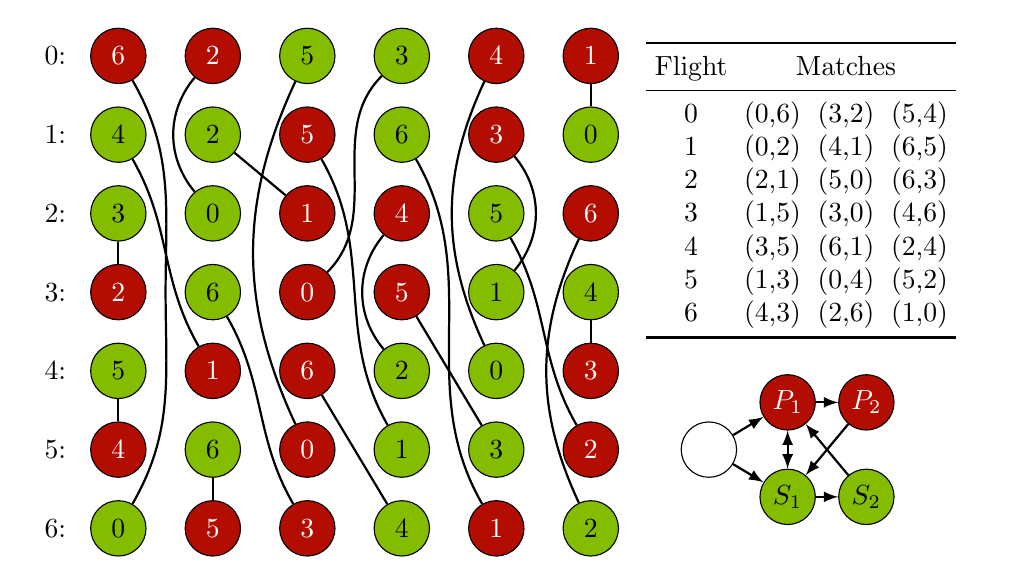
\begin{tikzpicture}
        \begin{scope}[every node/.style={minimum size=2em,inner sep=1}]
            \node (R0N)                                                at (0.4,  0) { 0: };
            \node (R00) [draw, circle, fill=uofgpillarbox, text=white] at ($(1.2 * 1,  0)$) { 6 };
            \node (R01) [draw, circle, fill=uofgpillarbox, text=white] at ($(1.2 * 2,  0)$) { 2 };
            \node (R02) [draw, circle, fill=uofglawn]                  at ($(1.2 * 3,  0)$) { 5 };
            \node (R03) [draw, circle, fill=uofglawn]                  at ($(1.2 * 4,  0)$) { 3 };
            \node (R04) [draw, circle, fill=uofgpillarbox, text=white] at ($(1.2 * 5,  0)$) { 4 };
            \node (R05) [draw, circle, fill=uofgpillarbox, text=white] at ($(1.2 * 6,  0)$) { 1 };

            \node (R1N)                                                at (0.4, -1) { 1: };
            \node (R10) [draw, circle, fill=uofglawn]                  at ($(1.2 * 1, -1)$) { 4 };
            \node (R11) [draw, circle, fill=uofglawn]                  at ($(1.2 * 2, -1)$) { 2 };
            \node (R12) [draw, circle, fill=uofgpillarbox, text=white] at ($(1.2 * 3, -1)$) { 5 };
            \node (R13) [draw, circle, fill=uofglawn]                  at ($(1.2 * 4, -1)$) { 6 };
            \node (R14) [draw, circle, fill=uofgpillarbox, text=white] at ($(1.2 * 5, -1)$) { 3 };
            \node (R15) [draw, circle, fill=uofglawn]                  at ($(1.2 * 6, -1)$) { 0 };

            \node (R2N)                                                at (0.4, -2) { 2: };
            \node (R20) [draw, circle, fill=uofglawn]                  at ($(1.2 * 1, -2)$) { 3 };
            \node (R21) [draw, circle, fill=uofglawn]                  at ($(1.2 * 2, -2)$) { 0 };
            \node (R22) [draw, circle, fill=uofgpillarbox, text=white] at ($(1.2 * 3, -2)$) { 1 };
            \node (R23) [draw, circle, fill=uofgpillarbox, text=white] at ($(1.2 * 4, -2)$) { 4 };
            \node (R24) [draw, circle, fill=uofglawn]                  at ($(1.2 * 5, -2)$) { 5 };
            \node (R25) [draw, circle, fill=uofgpillarbox, text=white] at ($(1.2 * 6, -2)$) { 6 };

            \node (R3N)                                                at (0.4, -3) { 3: };
            \node (R30) [draw, circle, fill=uofgpillarbox, text=white] at ($(1.2 * 1, -3)$) { 2 };
            \node (R31) [draw, circle, fill=uofglawn]                  at ($(1.2 * 2, -3)$) { 6 };
            \node (R32) [draw, circle, fill=uofgpillarbox, text=white] at ($(1.2 * 3, -3)$) { 0 };
            \node (R33) [draw, circle, fill=uofgpillarbox, text=white] at ($(1.2 * 4, -3)$) { 5 };
            \node (R34) [draw, circle, fill=uofglawn]                  at ($(1.2 * 5, -3)$) { 1 };
            \node (R35) [draw, circle, fill=uofglawn]                  at ($(1.2 * 6, -3)$) { 4 };

            \node (R4N)                                                at (0.4, -4) { 4: };
            \node (R40) [draw, circle, fill=uofglawn]                  at ($(1.2 * 1, -4)$) { 5 };
            \node (R41) [draw, circle, fill=uofgpillarbox, text=white] at ($(1.2 * 2, -4)$) { 1 };
            \node (R42) [draw, circle, fill=uofgpillarbox, text=white] at ($(1.2 * 3, -4)$) { 6 };
            \node (R43) [draw, circle, fill=uofglawn]                  at ($(1.2 * 4, -4)$) { 2 };
            \node (R44) [draw, circle, fill=uofglawn]                  at ($(1.2 * 5, -4)$) { 0 };
            \node (R45) [draw, circle, fill=uofgpillarbox, text=white] at ($(1.2 * 6, -4)$) { 3 };

            \node (R5N)                                                at (0.4, -5) { 5: };
            \node (R50) [draw, circle, fill=uofgpillarbox, text=white] at ($(1.2 * 1, -5)$) { 4 };
            \node (R51) [draw, circle, fill=uofglawn]                  at ($(1.2 * 2, -5)$) { 6 };
            \node (R52) [draw, circle, fill=uofgpillarbox, text=white] at ($(1.2 * 3, -5)$) { 0 };
            \node (R53) [draw, circle, fill=uofglawn]                  at ($(1.2 * 4, -5)$) { 1 };
            \node (R54) [draw, circle, fill=uofglawn]                  at ($(1.2 * 5, -5)$) { 3 };
            \node (R55) [draw, circle, fill=uofgpillarbox, text=white] at ($(1.2 * 6, -5)$) { 2 };

            \node (R6N)                                                at (0.4, -6) { 6: };
            \node (R60) [draw, circle, fill=uofglawn]                  at ($(1.2 * 1, -6)$) { 0 };
            \node (R61) [draw, circle, fill=uofgpillarbox, text=white] at ($(1.2 * 2, -6)$) { 5 };
            \node (R62) [draw, circle, fill=uofgpillarbox, text=white] at ($(1.2 * 3, -6)$) { 3 };
            \node (R63) [draw, circle, fill=uofglawn]                  at ($(1.2 * 4, -6)$) { 4 };
            \node (R64) [draw, circle, fill=uofgpillarbox, text=white] at ($(1.2 * 5, -6)$) { 1 };
            \node (R65) [draw, circle, fill=uofglawn]                  at ($(1.2 * 6, -6)$) { 2 };

            \draw [thick] (R00) to [out=300, in=90] ($(R30) + (0.6, 0)$) to [out=270, in=60] (R60);
            \draw [thick] (R10) to [out=300, in=120] (R41);
            \draw [thick] (R20) to                   (R30);
            \draw [thick] (R40) to                   (R50);

            \draw [thick] (R01) to [out=230, in=130] (R21);
            \draw [thick] (R11) to                   (R22);
            \draw [thick] (R31) to [out=300, in=120] (R62);
            \draw [thick] (R51) to                   (R61);

            \draw [thick] (R02) to [out=245, in=115] (R52);
            \draw [thick] (R12) to [out=300, in=120] (R53);
            \draw [thick] (R32) to [out=45,  in=225] (R03);
            \draw [thick] (R42) to                   (R63);

            \draw [thick] (R13) to [out=300, in=120] (R64);
            \draw [thick] (R23) to [out=230, in=130] (R43);
            \draw [thick] (R33) to                   (R54);

            \draw [thick] (R04) to [out=245, in=115] (R44);
            \draw [thick] (R14) to [out=310, in=50]  (R34);
            \draw [thick] (R24) to [out=300, in=120] (R55);

            \draw [thick] (R05) to                   (R15);
            \draw [thick] (R25) to [out=245, in=115] (R65);
            \draw [thick] (R35) to                   (R45);
        \end{scope}

        \begin{scope}[every node/.style={minimum size=2em,inner sep=1}, xshift=8.7cm, yshift=-5cm]
            \node (DFAI)  [draw, circle, fill=white]                     at (0,  0)   { \phantom{$P_1$} };
            \node (DFAP1) [draw, circle, fill=uofgpillarbox, text=white] at (1,  0.6) { $P_1$ };
            \node (DFAP2) [draw, circle, fill=uofgpillarbox, text=white] at (2,  0.6) { $P_2$ };
            \node (DFAS1) [draw, circle, fill=uofglawn]                  at (1, -0.6) { $S_1$ };
            \node (DFAS2) [draw, circle, fill=uofglawn]                  at (2, -0.6) { $S_2$ };

            \draw [->, >=latex, thick]  (DFAI)  to (DFAP1);
            \draw [->, >=latex, thick]  (DFAI)  to (DFAS1);
            \draw [->, >=latex, thick]  (DFAP1) to (DFAP2);
            \draw [<->, >=latex, thick] (DFAP1) to (DFAS1);
            \draw [->, >=latex, thick]  (DFAS1) to (DFAS2);
            \draw [->, >=latex, thick]  (DFAP2) to (DFAS1);
            \draw [->, >=latex, thick]  (DFAS2) to (DFAP1);
        \end{scope}

        \begin{scope}
            \node [anchor=north west] at (7.5, 0.3) {
                \begin{minipage}{4.5cm}
                    \centering
                    \setlength{\tabcolsep}{3pt}
                    \begin{tabular}{cccc}
                        \toprule
                        Flight & \multicolumn{3}{c}{Matches} \\ \midrule
                        0 & (0,6) & (3,2) & (5,4) \\
                        1 & (0,2) & (4,1) & (6,5) \\
                        2 & (2,1) & (5,0) & (6,3) \\
                        3 & (1,5) & (3,0) & (4,6) \\
                        4 & (3,5) & (6,1) & (2,4) \\
                        5 & (1,3) & (0,4) & (5,2) \\
                        6 & (4,3) & (2,6) & (1,0) \\ \bottomrule
                    \end{tabular}
                \end{minipage}
            };
        \end{scope}

    \end{tikzpicture}
    \caption{A pictorial representation of the orientation process, stage 4. Top right is the actual
        oriented schedule. Below that is the DFA to satisfy criterion~5. On the left is the zero/one
        variables, a row representing a skipper's sequence of competitors. An edge between variables
        corresponds to a matched pair, that must take different values.}\label{oriented}
\end{figure}

The final stage, stage 4, orients skippers within matches, such that they are either port (red) or
starboard (green). This is done to satisfy criteria~2 and~3, 5 and~8. A sketch of the constraint
model is given with a supporting diagram, Figure~\ref{oriented}.  A sequence of zero/one constrained
integer variables, of length $n-1$, is produced for each skipper. These correspond to the sequence
of skippers they meet in matches. For example, taking the schedule in Table~\ref{tab2}, skipper
$\sigma[{2}]$ meets skippers in order: 3,0,1,4,5,6, and skipper $\sigma[{5}]$ in the order
4,6,0,1,3,2.  Therefore, skipper $\sigma[{2}]$'s 4$^{th}$ variable must take a different value from
$\sigma[{5}]$'s 5$^{th}$ variable. There are summation constraints on each skipper to enforce
criteria~2 and~3 (equal number of port and starboard matches). Criterion~8 is enforced by posting
constraints such that in a match ($\sigma[{i}],\sigma[{j}]$) where $\abs*{i - j} = 1$, the higher
indexed skipper (lower ranked) is on the port side. A DFA constraint is posted for criterion~5
(restricting sequences of port and starboard assignments).

In Figure~\ref{oriented}, port is red and starboard green. The sequence of zero/one variables for
each skipper is shown on the left. Bottom right is the DFA, and top right is the final schedule
produced from stages 1 to 4. The schedule has 6 boat changes and a maximum imbalance of 1. Three
days CPU time was devoted to stages 1 and 2. Stages 3 and 4 completed in 15 milliseconds. The
schedule presented here is new, not appearing in the example schedules provided in the manual
\cite{isaf}.

\section{Sample Schedules}\label{sec:samples}

We present four pairs of schedules. The first pair is for 8 skippers and 6 boats, one published by
ISAF, the other generated by us. Next, we present two new schedules, not appearing in the ISAF
manual, for 9 skippers and 6 boats and 9 skippers with 8 boats, then 10 skippers and 6 boats, again
both published by ISAF and generated by us. Finally, we show what is a relatively easy problem, 8 skippers
and 8 boats.  For each of our schedules (with the exception of the latter ``easy-8'' problem), we used 1 day
CPU time for the first stage (minimising boat changes) then a further 2 days to minimise imbalance.
Stages 3 and 4 (renaming and orientation) completed in less than a second.

\begin{figure}[b]
\begin{minipage}[t]{0.48\textwidth}
    \centering
\begin{tabular}{cccc}
        \toprule
        Flight & \multicolumn{3}{c}{Matches} \\ \midrule
        0 & (5,2) & (4,3) & (1,6) \\
        1 & (4,2)  & (6,5) & (3,1) \\
        2 & (6,4) & (2,1) & (3,5) \\
        3 & (6,2) & (5,0) & (1,7) \\
        4 & (5,1) & (0,6) & (2,7) \\
        5 & (7,5) & (2,0) & (6,3) \\
        6 & (0,7) & (4,1) & (3,2) \\
       7 & (7,4)  & (0,3) &  \\
       8 & (4,0)  & (7,3) &  \\
       9 & (5,4)  & (7,6) & (1,0) \\ \bottomrule
    \end{tabular}
\label{08-06a}
\end{minipage}
\hfill
\begin{minipage}[t]{0.48\textwidth}
    \centering
\begin{tabular}{cccc}
        \toprule
        Flight & \multicolumn{3}{c}{Matches} \\ \midrule
        0 & (2,7) & (3,0) & (5,4) \\
        1 & (0,2)  & (4,3) & (7,5) \\
        2 & (0,4) & (7,6) & (5,3) \\
        3 & (4,6) & (5,0) & (3,1) \\
        4 & (6,5) & (3,2) & (1,4) \\
        5 & (6,3) & (4,7) & (2,1) \\
        6 & (7,3) & (1,6) & (4,2) \\
       7 & (7,1)  & (2,5) & (6,0) \\
       8 & (5,1)  & (0,7) & (6,2) \\
       9 & (1,0)  & & \\ \bottomrule
    \end{tabular}
\label{08-06b}
\end{minipage}
\caption{Schedules for 8 skippers and 6 boats. On the left, the published ISAF schedule (illegal),
and on the right is our schedule.}
\label{08-06}
\end{figure}

\paragraph{8 skippers and 6 boats:} We first analyse the ISAF schedule, Table~\ref{08-06} on the
left. Criterion~4 (skippers in last match in a flight cannot be first in next flight) is violated on
3 occasions (skipper 1 in flight 3, skipper 7 in flight 4, skipper 0 in flight 7). Criterion~5 (no
more than two consecutive port or starboard assignments) is violated for skipper 6 (flights 1 to 3)
and skipper 7 (flights 7 to 9). Criterion~6 (imbalance) is violated for skippers 6 and 8. Criterion~12  (new
boats do not sail first) is violated in flight 9 for skipper 5. Finally, the schedule has 8 boat
changes. Our schedule, Table~\ref{08-06} on the right, respects all criteria and has 6 boat changes
and a maximum imbalance of 1.

\paragraph{9 skippers:} Two new schedules are presented in Table~\ref{09}, on the left for 6 boats
and on the right for 8 boats. Neither of these schedules appear in the ISAF Umpires' Manual. Both
schedules respect all criteria. For 6 boats there are 8 boat changes (no skipper making more than 1
boat change) and a maximum imbalance of 2. For 8 boats there are again 8 boat changes, no skipper
with more than 1 boat change, and each skipper 4 times on starboard side and 4 on port side.

\begin{figure}[h]
\begin{minipage}[t]{0.48\textwidth}
\centering
\begin{tabular}{cccc}
        \toprule
        Flight & \multicolumn{3}{c}{Matches} \\ \midrule
        0 & (0,7) & (3,2) & (5,4) \\
        1 & (0,2) & (7,4) & (5,3) \\
        2 & (4,0) & (7,3) & (2,5) \\
        3 & (3,0) & (2,4) & (6,5) \\
        4 & (4,3) & (5,1) & (8,6) \\
        5 & (3,1) & (6,2) & (4,8) \\
        6 & (6,3) & (1,4) & (8,2) \\
        7 & (4,6) & (2,7) & (1,8) \\
        8 & (7,6) & (0,8) & (2,1) \\
        9 & (8,7) & (5,0) & (6,1) \\
        10 & (8,5) & (1,7) & (0,6) \\
        11 & (7,5) & (3,8) & (1,0) \\ \bottomrule
    \end{tabular}
\centering
\label{09-06}
\end{minipage}
\hfill
\begin{minipage}[t]{0.48\textwidth}
\centering
\begin{tabular}{ccccc}
        \toprule
        Flight & \multicolumn{4}{c}{Matches} \\ \midrule
        0 & (0,6) & (3,2) & (5,4) & (1,7) \\
        1 & (2,0) & (6,3) & (4,1) & (8,7) \\
        2 & (6,4) & (0,5) & (7,2) & (3,8) \\
        3 & (4,7) & (1,8) & (0,3) & (5,2) \\
        4 & (3,1) & (7,5) & (8,0) & (2,6) \\
        5 & (3,7) & (4,8) & (2,1) & (6,5) \\
        6 & (8,2) & (1,6) & (5,3) & (0,4) \\
        7 & (5,1) & (7,0) & (6,8) & (4,3) \\
        8 & (8,5) & (2,4) & (7,6) & (1,0) \\ \bottomrule
        & & & & \\
        & & & & \\
        & & & & \\
    \end{tabular}
\label{09-08}
\end{minipage}
\caption{Two new schedules. On the left, 9 skippers and 6 boats, and on the right 9 skippers and 8 boats.}
\label{09}
\end{figure}

\paragraph{10 skippers and 6 boats:} Table \ref{10-06} shows the ISAF schedule on the left for 10
skippers and 6 boats and on the right, our schedule.  The ISAF schedule violates criterion~5 (no more
than 2 consecutive port or starboard assignments) ten times (twice for skippers 0, 1 and 6 and once
for skippers 3, 7, 8 and 9).  Criterion~12 (new boats do not sail first) is violated 7 times (in
flight 3 for skippers 6 and 2, flight 5 for skipper 8, flight 6 for skipper 7, flight 8 for skipper
1, flight 9 for skipper 4 and flight 12 for skipper 4 again). There are 22 boat changes, with the
minimum changes for a skipper being 1 and the maximum 3. Our schedule, right of Table \ref{10-06},
satisfies all criteria, has 12 boat changes with the minimum changes for a skipper being 0 and the
maximum 2, and a maximum imbalance of 1.

\begin{figure}[h]
\begin{minipage}[t]{0.48\textwidth}
    \centering
\begin{tabular}{cccc}
 \toprule
Flight & \multicolumn{3}{c}{Matches} \\ \midrule
0 & (8,3) &  (1,7) &  (0,9) \\
1 & (7,3) &  (0,8) &  (1,9) \\
2 & (0,7) &  (9,3) &  (1,8) \\
3 & (6,2) &  (5,0) &  (7,4) \\
4 & (5,2) &  (6,4) &  (3,0) \\
5 & (8,6) &  (2,9) &  (4,1) \\
6 & (7,2) &  (4,8) &  (9,6) \\
7 & (2,4) &  (0,6) &  (7,5) \\
8 & (6,1) &  (5,9) &  (8,2) \\
9 & (9,4) &  (8,7) &  (6,5) \\
10 & (9,7) &  (6,3) &  (8,5) \\
11 & (7,6) &  (3,1) &  (9,8) \\
12 & (4,3) &  (5,1) &  (2,0) \\
13 & (3,5) &  (4,0) &  (2,1) \\
14 & (5,4) &  (3,2) &  (1,0) \\ \bottomrule
\end{tabular}
\label{10-06a}
\end{minipage}
\hfill
\begin{minipage}[t]{0.48\textwidth}
\centering
\begin{tabular}{ccccc}
\toprule
Flight & \multicolumn{3}{c}{Matches} \\ \midrule
0 & (4,7) & (3,2) & (0,5) \\
1 & (2,4) & (7,0) & (3,5) \\
2 & (0,4) & (7,3) & (5,2) \\
3 & (4,3) & (0,2) & (5,7) \\
4 & (3,0) & (6,5) & (2,7) \\
5 & (6,3) & (7,1) & (8,2) \\
6 & (7,6) & (2,1) & (9,8) \\
7 & (2,6) & (8,7) & (4,9) \\
8 & (6,8) & (1,4) & (7,9) \\
9 & (8,1) & (5,4) & (9,6) \\
10 & (5,1) & (9,2) & (4,6) \\
11 & (1,9) & (6,0) & (8,4) \\
12 & (0,9) & (3,8) & (6,1) \\
13 & (8,0) & (9,5) & (1,3) \\
14 & (5,8) & (9,3) & (1,0) \\ \bottomrule
\end{tabular}
\label{10-06b}
\end{minipage}
\caption{Schedules for 10 skippers and 6 boats. On the left, the ISAF published schedule (illegal),
and on the right, our schedule.}
\label{10-06}
\end{figure}

\paragraph{8 skippers and 8 boats (easy-8):} Table \ref{08-08} shows the ISAF schedule on the right
for 8 skippers and 8 boats and on the right, our schedule.  The ISAF schedule violates criterion~4
(last match in a flight cannot be first in next flight) for skipper 5 in flights 1 and 2. Also,
criterion 5 (no skipper should have more than 2 consecutive port or starboard assignments) is
violated for skippers 0, 1, 3, 4 and 6. Furthermore, skipper 1 appears in the last match of four
flights resulting in significant imbalance. Our schedule, on the right, satisfies all criteria, is
optimal (maximum imbalance of 1) and took less than 10 seconds in total (all stages) to produce.

\begin{figure}[h]
\begin{minipage}[t]{0.48\textwidth}
    \centering
\begin{tabular}{ccccc}
        \toprule
        Flight & \multicolumn{4}{c}{Matches} \\ \midrule
0 & (5,2) & (4,3) & (1,6) & (0,7) \\
1 & (2,4) & (0,6) & (1,7) & (5,3) \\
2 & (0,5) & (7,2) & (6,3) & (4,1) \\
3 & (7,3) & (5,1) & (4,0) & (6,2) \\
4 & (3,0) & (4,7) & (6,5) & (2,1) \\
5 & (6,4) & (7,5) & (2,0) & (3,1) \\
6 & (7,6) & (5,4) & (3,2) & (1,0) \\ \bottomrule
    \end{tabular}
\label{08-08a}
\end{minipage}
\hfill
\begin{minipage}[t]{0.48\textwidth}
    \centering
\begin{tabular}{ccccc}
        \toprule
        Flight & \multicolumn{4}{c}{Matches} \\ \midrule
0 & (4,3) & (2,0) & (1,5) & (7,6) \\
1 & (3,2) & (0,4) & (6,1) & (5,7) \\ 
2 & (4,1) & (7,3) & (5,2) & (0,6) \\
3 & (1,7) & (6,5) & (3,0) & (2,4) \\ 
4 & (0,5) & (4,6) & (7,2) & (3,1) \\
5 & (7,0) & (2,1) & (6,3) & (5,4) \\ 
6 & (6,2) & (5,3) & (4,7) & (1,0) \\ \bottomrule
    \end{tabular}
\label{08-08b}
\end{minipage}
\caption{Schedules for 8 skippers and 8 boats. On the left, the published ISAF schedule (illegal),
and on the right, our schedule.}
\label{08-08}
\end{figure}

\section{Discussion}

It was anticipated that this problem would be easy to model. This naivety was due to the use of the
term ``round-robin'' for these schedules, leading us to believe that we could use some of the models
already in the literature \cite{trick2002,trick2008,henz2004}. This naivety slowly dissolved as
we addressed more and more of the ISAF criteria. A number of models we produced were scrapped due to
misunderstanding about the actual problem, i.e.\ a communication problem between the authors.
Eventually this was resolved by presenting the majority of the criteria as a deterministic finite
automaton. This became our Rosetta Stone, with the surprising benefit that it not only improved the
teams communications, it was also a constraint!

The staged approach was taken cautiously. We expected that isolating the orientation of schedules as
a post-process might leave us with a hard or insoluble problem. So far, every schedule we have
produced has been oriented with very little search, typically taking less than a second.

We used the choco constraint programming toolkit and one of our goals was to use only toolkit
constraints, i.e.\ we wanted to see how far we could go without implementing our own specialised
constraints. We are pleased to say that we did not have to do anything out of the box, although we
did feel that we had used just about every constraint there was.

There are many redundant variables in our model. One of our first valid models was essentially that
shown in Figure~\ref{skipper5}, and did not use $\modMatch$ and $\match$ variables. Performance was
hopeless, struggling to produce a 7 skipper 6 boat schedule in days. The $\modMatch$ and $\match$
variables were added. This improved domain filtering, and a flattened $\match$ array was used as
decision variables. That is, the decisions where ``when do we schedule this match?''.  At this point
we had not yet produced a 9 skipper 6 boat schedule and we suspected that the combined criteria
might exclude such a schedule. A non-constraint model was developed, primarily
to attempt to prove that there was no schedule for 9 skippers with 6 boats. This program used a
backtracking search with decision variables being positions within flights, i.e.\ time slots being
assigned to matches. At the top of search, the matches in the first flight were set, and symmetry
breaking was used to reduce the number of legal second flights. A solution was found in seconds!
With this experience we added in the $\timeVar$ variables, channeled these into the existing model
and used these as decision variables, i.e.\ the question now was ``what match will we do now?''. We
also anchored the matches in the first flight. With these changes we began to produce schedules in
acceptable time. The model was then built upon, incrementally adding criteria. This took a
surprisingly short amount of time, sometimes minutes of coding to add in a new feature. The model
was then enhanced so that it would address optimisation rather than just satisfaction, again a
trivial programming task.

We have only reported a handful of our schedules, however there are missing schedules. Examples of
these missing schedules are 10 skippers and 8 boats, 11 skippers with fewer than 10 boats, 12
skippers and 8 boats, 13 skippers and 8 boats and 14 skippers with fewer than 10 boats. None of these
schedules have been published by the ISAF, although we expect that they can be produced by
selectively violating some of constraints. We have also not yet encoded criterion~7, addressing the
situation of 10 or more boats. To do this we will have to modify the DFA constraint used in the
first two stages.

\section{Conclusion}\label{sec:conclusions}

\begin{figure}[tb]
    \centering
    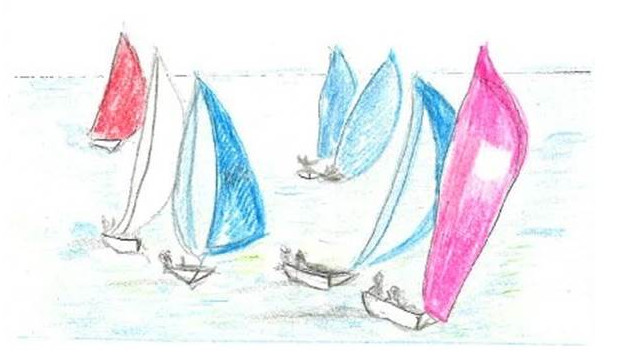
\includegraphics[keepaspectratio=true,width=4.6in]{dinghy.jpg}
\caption{Scene from an imaginary dinghy race.}
\label{dinghy}
\end{figure}

We have produced new and better match race schedules. These schedules can be used by anyone that
competes under the criteria published by ISAF. Our schedules can be downloaded as blank schedules
and then populated with the names of the actual competing skippers.

So, why did we use constraint programming? The answer is obvious:  we are constraint programmers, or
to borrow Mark Twain's words ``To a man with a hammer, everything looks like a nail''. But actually,
constraint programming has been a good way to go. From an engineering perspective, it has allowed us
to prototype solutions quickly and to build solutions incrementally. There is also an advantage that
we might exploit in the future: we can now investigate the effect different criteria have on our
ability to produce schedules and how relaxation of those affect optimisation criteria. That is, the
constraint program might be used to design the next set of criteria for match race schedules, or
allow the event organiser to decide which criteria to sacrifice to ensure a faster schedule with
fewer boat changes.

\bibliographystyle{plain}
\bibliography{bib}

\end{document}
